
\chapter{Calibration of the CMS Hadron Forward Calorimeter} \label{chapter:hf}

\section{Introduction and Motivation}
During the First Long Shutdown (LS1) of the Large Hadron Collider (LHC), Hadron Forward (HF) Calorimeters have undergone substantial hardware upgrade: the
new HF Photo Multiplier Tubes (PMTs) have been installed and the part of the readout electronics has been replaced. Therefore, the detector had to be recommissioned in preparation for the Run II datataking campaign. In order to establish the Calibration Coefficients (CCs) for the HF Calorimeter with the new PMTs, three sourcing campaigns have been performed: HF- October 2013, HF+ April 2014, and HF- July 2014.

In this chapter the procedure and results of the performed calibration are presented.

% In this paper, we specifically concentrate on
% discussing the results of HF Source Calibration. In Section 2, a brief description of HF
% calorimeter is presented. Section 3 provides a detailed description of the
% calibration workflow, including the description of the source driver system and
% HF Data Acquisition System (DAQ). In this section we also provide a description of all Sourcing Campaigns and outline issues experienced during the data taking. In Section 4, we thoroughly outline the analysis procedure used, and then the results of each sourcing campaign performed
% during the LS1 are presented in the Section 5, Finally, we conclude summarizing the results of Sourcing Campaign during LS1.

\section{Description of HF Calorimeters}

The Hadron Forward (HF) calorimeters in the Compact Muon Solenoid (CMS)
experiment at the Large Hadron Collider (LHC) cover a large pseudorapidity
range, $3 \le |\eta| \le 5$, and thus significantly improve jet detection and the missing transverse energy resolution which are essential in top quark production studies, Standard Model Higgs, and all SUSY particle searches~\cite{CMSTP:1994,CMSTP:1997}.

The CMS has two hadronic forward calorimeters, HF- and HF+, each essentially a cylindrical steel structure with an inner radius of 12.5 cm to accommodate the beam pipe, an outer radius of 130.0 cm, and with the front face located 11.15 m from the interaction point. Both calorimeters are wrapped by hermetic radiation shielding of 40 cm thick steel, 40 cm of concrete, and 5 cm of polyethylene, with a large steel plug in the back of each detector.

\begin{figure}[!h]
   \begin{center}
      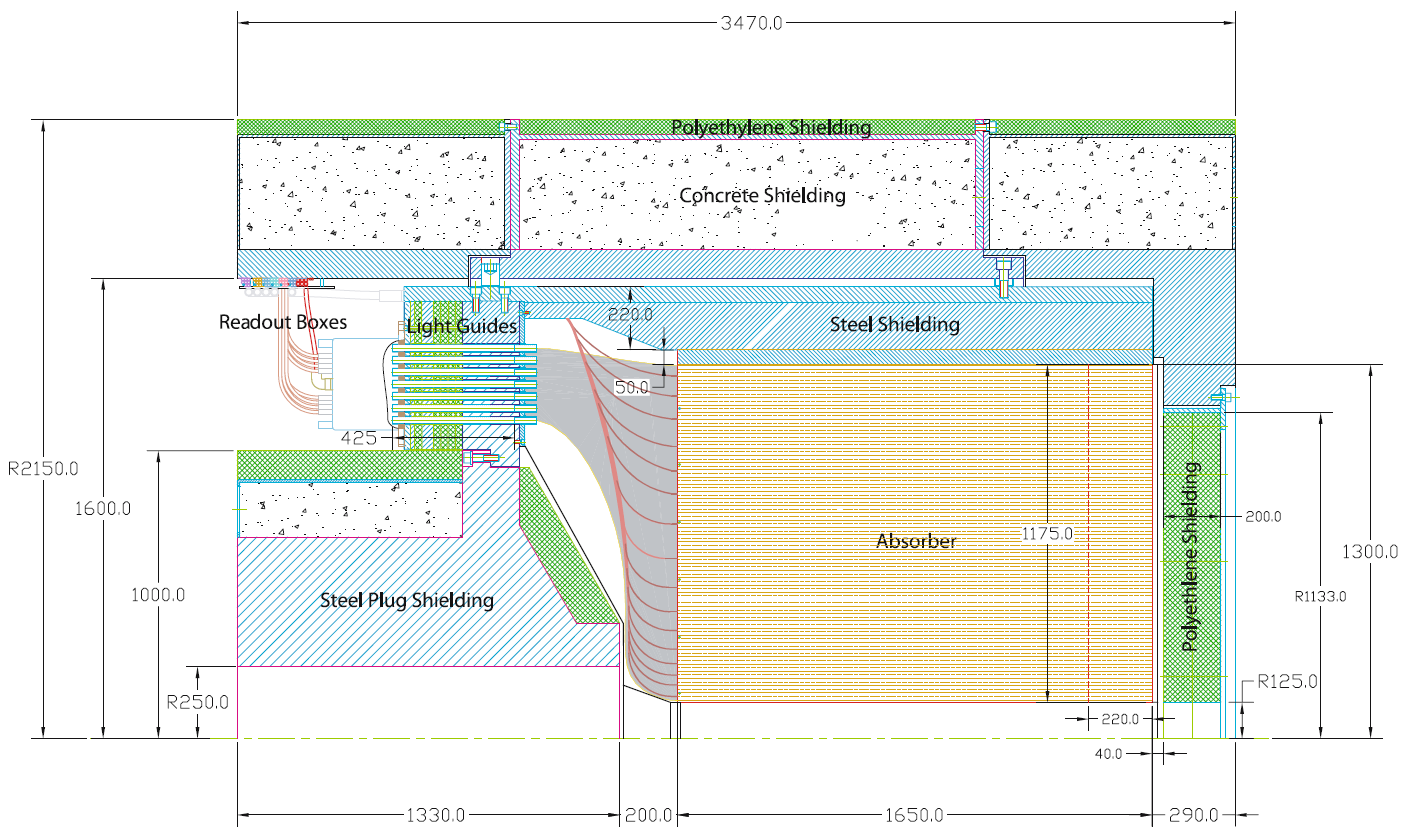
\includegraphics[width=1.\textwidth]{figures/ch_hfcalibration/HF_Calorimeter.png}
      \caption{Cross section of the HF calorimeter. IP is to the right}
      \label{fig:hf_description_crosssectionview}
   \end{center}
\end{figure}

Figure~\ref{fig:hf_description_crosssectionview} displays a cross sectional view of an HF calorimeter. Each HF side is azimuthally subdivided into 18 20 de wedges composed of 5 mm thick grooved steel plates that perform as absorbers. The plate grooves run parallel to the beam line and are spaced 5.0 $\pm$ 0.1 mm center-to-center, each housing a single optical fiber. Each fiber consists of a fused-silica, also referred to as quartz, core of 600 $\pm$ 10 mum diameter, layered to an outer diameter of 630 $^{+5}_{-10}$ mum with polymer hard-clad, and surrounded to a final diameter of 800 $\pm$ 30 mum with protective acrylate buffer. The optical attenuation for each fiber scales as $a(\lambda)(D/D_0)^{b(\lambda)}$, where $a$ and $b$ characterize radiation hardness, $D$ is the accumulated dose, and $D_0$ is a reference dose (100 MRad)~\cite{HFCC:2008}. Each
wedge's fibers are bundled to form 24 towers, each with 0.175 x 0.175 ($\Delta\eta$ x $\Delta\phi$) angular span, with exception in angular span for the 2 towers formed closest to the beam pipe. The bundled fibers are held in ferrules that illuminate one end of air-core light guides penetrating shielding of steel, lead, and polyethylene necessary for the readout boxes. The air-core light
guides are hollow tubes inlined with highly reflective metal-coated sheets and are coupled to standard bialkaline, 8-stage R7525 Hamamatsu photomultiplier tubes (PMT) with a borosilicate glass window. During LS1 R7525 PMTs (Old) were replaced by metal case Hamamatsu R7600 PMTs (New), which have a thinner front window.

Cherenkov light forms the signal from charged shower particles above the Cherenkov threshold (E $\ge$ 190keV for electrons), optimizing the HF calorimeter's sensitivity to the electromagnetic component of showers~\cite{Akchurin:2955}. Light incident upon the core-cladding interface above the critical angle (71 de) contributes to the signal, although a small fraction of light is captured in the numerical aperature (NA = 0.33 $\pm$ 0.02) and only half reaches the PMT photocathode. Since the calorimeter is most sensitive to the electromagnetic component of showers, two different lengths of optical fibers are inserted into the absorbers and connected to separate PMTs. Half of all fibers in each calorimeter extend the full depth of the absorber (165 cm $\approx$ 10 $\lambda_I$), while the other half starts 22 cm from the front end. These depths are chosen because a large fraction of energy from electrons or photons are deposited within the first 22 cm of the absorber's front end, while energy from hadronic showers can be deposited throughout the absorber. The naming convention for these two depths of fibers is EM (or L) for the long fibers collecting the total signal and H (or S) for the short fibers collecting the signal from beyond the first 22 cm. Therefore, with 24 towers per wedge
and 2 PMTs per tower, a single readout box housing 24 PMTs services half a wedge (10 de).

In order to uniformly collect data throughout each wedge between EM and H fiber bundles, each absorber groove is filled with alternating EM or H fibers. For the purpose of calibrating the energy readout from each calorimeter, a groove in the center of each tower has its corresponding EM or H fiber replaced with a hollow 15 gauge stainless steel tube with inner and outer diameters of 0.97 mm and 1.32 mm, respectively, referred to as a source tube. Due to the geometry and  varying dimensions of certain towers, there can be more than one groove housing a source tube in order to calibrate sufficiently, especially for higher $\eta$ towers.

\begin{figure}[!h]
   \begin{center}
      \subfigure[]{
         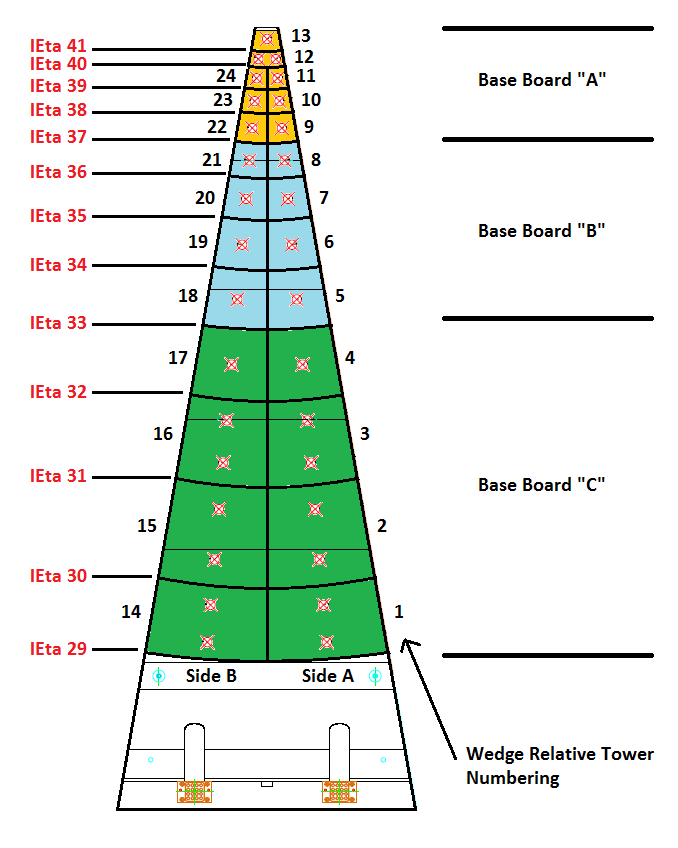
\includegraphics[width=.65\textwidth]{figures/ch_hfcalibration/HFWedge.png}
      }
      \caption{Diagram of a single HF calorimeter wedge}
      \label{fig:hf_description_wedgediagram}
   \end{center}
\end{figure}

Figure~\ref{fig:hf_description_wedgediagram} displays a transverse segmentation of a single wedge with all 24 towers and 31 source tubes. It can be seen in Figure~\ref{fig:hf_description_wedgediagram} that the geometry of each tower changes significantly between high $\eta$ index and low $\eta$ index; therefore, it is expected that the energy deposited into each tower by the passing radioactive source varies.

\begin{table}[!h] \centering \scalebox{1.10}{
  \begin{tabular}{|c|c|c|c|}
  \hline
  Tube & Mismatch & Match & Unc. \\
  \hline
  \hline
  1(14)A & 0.917 & 0.840 & 0.017 \\
  1(14)B & 0.909 & 0.833 & 0.017 \\
  2(15)A & 0.945 & 0.866 & 0.009 \\
  2(15)B & 0.938 & 0.859 & 0.009 \\
  3(16)A & 0.925 & 0.846 & 0.013 \\
  3(16)B & 0.908 & 0.829 & 0.015 \\
  4(17)  & 0.930 & 0.851 & 0.002 \\
  5(18)  & 0.889 & 0.810 & 0.003 \\
  6(19)  & 0.847 & 0.772 & 0.004 \\
  7(20)  & 0.789 & 0.713 & 0.006 \\
  8(21)  & 0.715 & 0.633 & 0.018 \\
  9(22)  & 0.646 & 0.572 & 0.006 \\
  10(23) & 0.597 & 0.516 & 0.013 \\
  11(24) & 0.498 & 0.425 & 0.023 \\
  12A(B) & 0.413 & 0.331 & 0.056 \\
  13     & 0.588 & 0.510 & 0.023 \\
  \hline
  \end{tabular}}
  \caption{Geometric correction factors for each tower's energy containment for a radioactive source
  passing through a given source tube. The value depends on what source tube contains the radioactive
  source and whether there is a match between the type of optical fiber that the source tube replaced.}
  \label{tab:hf_description_gcfactors}
\end{table}

The radioactive source excites a small region of the absorber within its immediate vicinity - 90\% of the signal output originates from a region within 3 cm of the source, with the closest optical fibers to the source contributing the most output. When performing radioactive source calibration, each tower is sourced
and analyzed separate from its neighbors; therefore, geometric correction factors must be applied to the signal output from each tower to account for the energy that escapes into neighboring towers. Monte Carlo techniques are used to account both for the energy leakage of a given tower as well as the relative position of the source tube with respect to the optical fibers (the source tubes replaced
either an EM or H type optical fiber). Table~\ref{tab:hf_description_gcfactors} lists the geometric correction factors for each tower's energy containment with respect to the type of optical fiber and the source tube replaced.

% Figure~\ref{fig:HF_Grooves} shows a matrix of groove types which identifies the  optical fiber type that was replaced by a source tube for each tower.

% \begin{figure}[!h]
%    \begin{center}
%       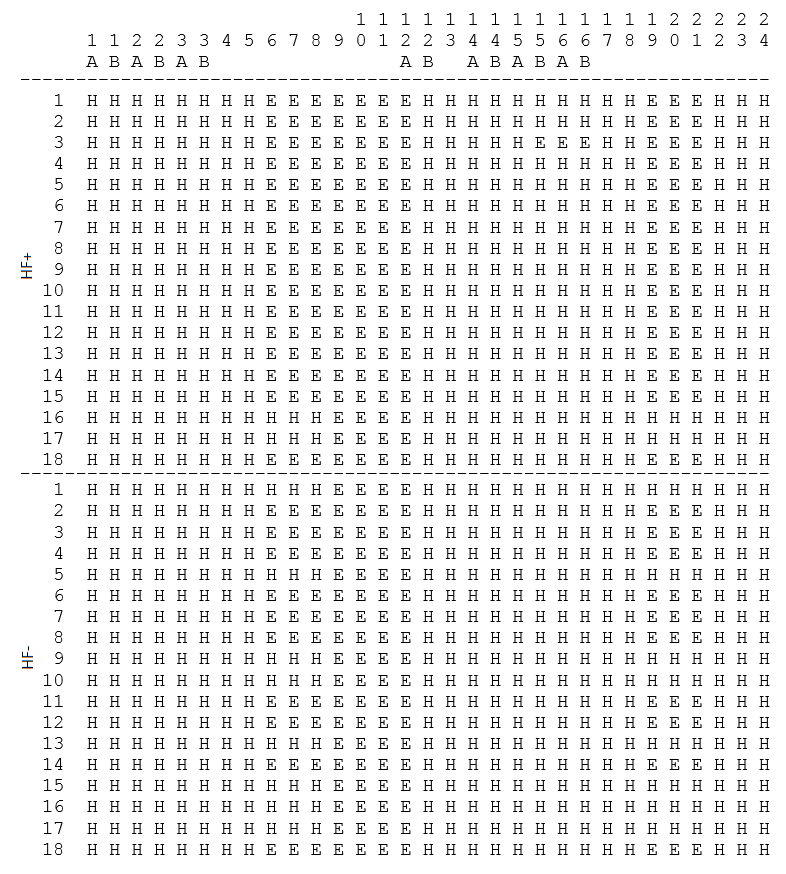
\includegraphics[width=1.\textwidth]{figures/ch_hfcalibration/Groove_Type.png}
%       \caption{Matrix of groove types that each source tube occupies within both HF
%       Calorimeters. First column is wedge number, ranging from 1-18 for each calorimeter.
%       The top row lists each source tube number for a given wedge, ranging from 1A-24.
%       Within the matrix, an E means that the source tube replaced an EM optical fiber, and
%       a H means the source tube replaced a H optical fiber.}
%       \label{fig:HF_Grooves}
%    \end{center}
% \end{figure}
\section{Experimental Setup}

\subsection{Source Driver System}
To perform calibration of the calorimeter with a radioactive source, a
specialized source driver system has been developed. It includes devices capable of inserting a long thin wire, approximately 11 m long, tipped with a point-like radioactive source into the HF source tubes embedded in the calorimeter. As the radioactive source moves through the HF absorber, gamma rays are generated and consequently create Compton electrons, which in turn can generate Cherenkov photons inside the quartz fibers if they exceed the Cherenkov threshold. With the new HF PMTs, the quantum efficiency is such that only 30\% of the photons reaching the PMT cathode face will actually be converted into the read out signal.

The thin wire, referred to as the source wire, used by the system is made of
stainless steel and has an inner and outer diameter of 0.406 mm and 0.711 mm,
respectively. The end of the wire that penetrates the HF absorber, the front end,
is melted shut, shaped into a bullet nose, and chemically plated to reduce friction. The point-like radioactive source is inserted into the opposite end of
the wire, the back end, and held in place against the front end by a fine steel
piano wire. The outer source wire and inner piano wire are then crimped together at the back end in order to fix the position of the radioactive source.

A Lexan polycarbonate reel, belt driven by a DC reversible electric motor, is used
to insert or retract the source wire into or out of the calorimeter's source tubes.
The calorimeter's source tubes are coupled to acetal plastic tubing to mediate the
transfer of the source wire from the source driver into the absorber. The
transition between the plastic tube and the metal source tube typically involve
small-angle conical holes in brass that channel the source wire to the source tube.

\begin{figure}[!h]
   \begin{center}
      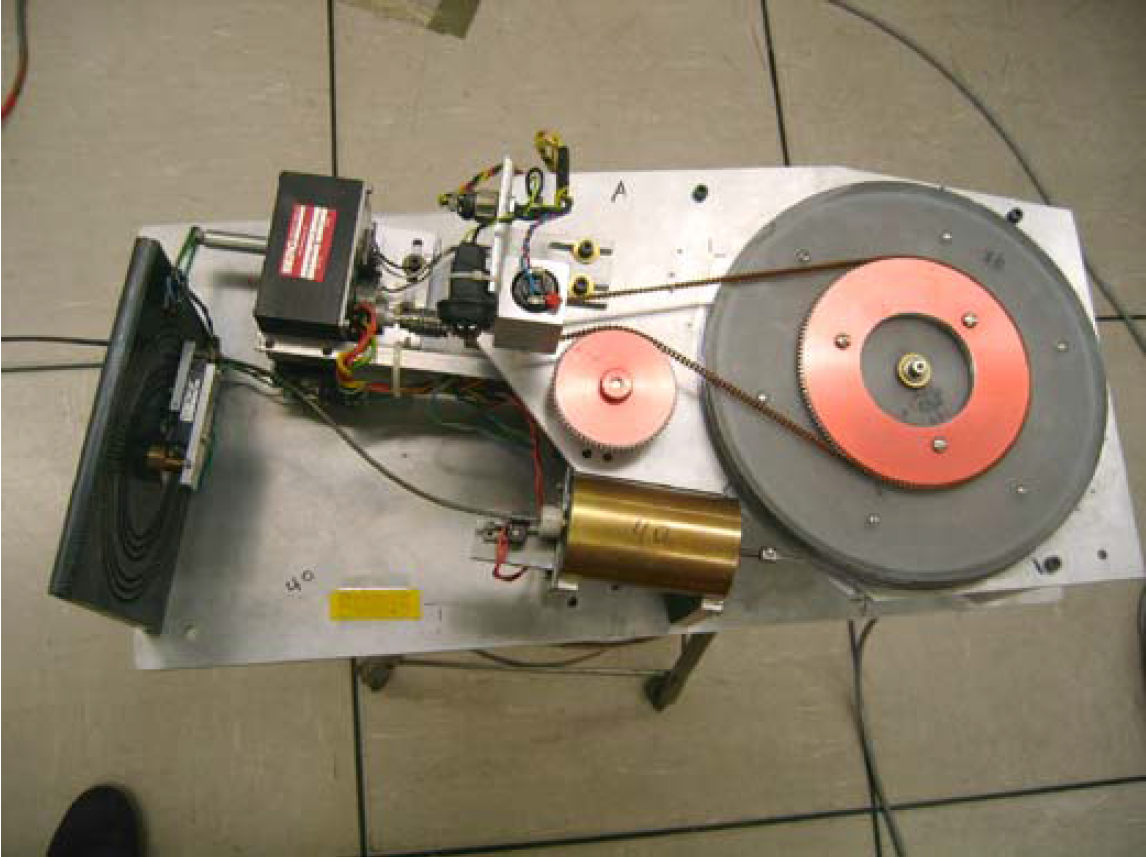
\includegraphics[width=.5\textwidth]{figures/ch_hfcalibration/Source_Driver.png}
      \caption{Source Driver System}
      \label{fig:hf_expsetup_sourcedriver}
   \end{center}
\end{figure}

The driver system also contains an additional electric motor that functions to
select the source tube into which to direct the source wire, an action referred
to as indexing. The position of the radioactive source, relative to the source
driver and referred to as the reel position, is provided by an optical rotary
encoder read out by industrial batch counters. Typical speeds at which the
radioactive source may be inserted or retracted by the driver are between 5 and
15 cm/s. Figure~\ref{fig:hf_expsetup_sourcedriver} displays the source driver configuration.

\subsection{HF DAQ Description}
The PMT analog signals are read out by QIEs, standing for charge (Q),
integration (I), and encode (E). Each such QIE has 3 differential inputs, which
allows to digitize 3 PMTs simultaneously. Differential inputs are used to subtract
any externally induced noise in signal cables. Each QIE has also 1 fiber-optic
output, which transfers the digitized information to HTRs (HCAL Trigger and
Readout). The output of 8 QIEs (8 fibers) is bundled up into 1 cabel, which in
turn is connnected to either top or bottom half of the HTR, equaling 16 QIEs
(16 fibers) per HTR. Therefore, each HTR receives input from 48 PMTs: 24 PMTs for
each tower's HAD channel and 24 PMTs for each tower's EM channel.

A large dynamic range in PMT signal processing is acquired using
a multi-range technique. The input current is sumulatenously integrated on all
four ranges, and comparators are used to isolate the lowest range that is not at
full scale. The selected voltage representing the integrated charge is then put
through an on-chip piecewise linear Flash ADC (Analogue to Digital Converter),
with bins weighted according to the time slice (TS) firmware used. For 1TS, 15
bins are weighted 1, 7 bins weighted 2, 4 bins weighted 3, 3 bins weighted 4,
and 3 bins weighted 5, providing a range from 0 to 63 ADC counts, with the last
bin (overflow bin) containing all charge above 63 ADC counts. For 2TS, 10 bins
are weighted 1, 6 bins weighted 2, 5 bins weighted 4, 5 bins weighted 8, 3 bins
weighted 16, 2 bins weighted 32, and 1 bin weighted 62, providing a range from
0 to 194 ADC counts, with the overflow bin containing all charge above 194 ADC
counts. Operations are time multiplexed and pipelined to allow signals to
settle and to make the reset interval the same as the inegration interval.
Clocking is provided at the frequency of 40 MHz, with a latency of
100 ns, as the pipeline is four clock cycles deep. Each QIE contains a
set of four capacitors, and only one capacitor is acquiring charge during a
given clock cycle. The output is a 5-bit mantissa representing the voltage on
the particular capacitor, and a 2-bit exponent indicating the range
represented by a coded address of the capacitor.

The firmware implemented during radioactive source data collecting uses a
given TS histogramming mode and operating voltage (OV). In the histogramming
mode, the absorber's response charge is represented across 32 histogram bins,
with the final bin, Bin 32, being the overflow bin containing all data with
charge beyond the particular range. For 1TS firmware, each TS was recorded in
the histogram. For 2TS firmware, two adjacent TS segments were compared, and
the maximum output from the pair was recorded in the histogram. To accomodate
the 2TS maximum outputs, the expanded QIE bin range described above was used
with respect to 1TS.

Each capacitor from a QIE set fills a separate histogram at the sampling rate,
i.e. latent cycle, and once $6.5535 x 10^4$ samples are collected the histogram
is read out by the DAQ, two HTR fibers from each HTR half at a time. Data is
saved by event, each event containing the histograms read out by all powered HTR
halves - a given PMT's output is stored in every fourth event. This provides
that each event represents 6.55 ms of source data. For 1TS, each sample
was collected over 25 ns, and for 2TS each sample was collected over
50 ns.
\section{Sourcing Campaigns}
A $^{60}$Co radioactive source, RP4118 with a measured activity of 83.46 $\pm$
0.10 MBq on 14 September 2012, was used to produce the signal readout
during the three sourcing campaigns: HF- in October 2013 with the old PMTs still
installed; HF+ in April 2014 with new PMTs installed; and HF- in July 2014 with
new PMTs installed. First, sourcing with the old PMTs was performed to extract
the source energy deposition in terms of HF calibration during Run 1. Second, new PMTs were installed and commissioned. Finally, the sourcing was performed with the newly installed hardware and previously extracted source energy deposition was applied to compute the HF gains. Several OVs, which are different from the Voltage that HF is being planned to be operated at during Run II (OV2), were used depending on the histogramming mode (1 TS or 2 TS) as it was important on one hand to take into account the limitations of the QIE range. On the other hand, we have to have sufficient PMT gain not to lose events under the pedestal peak. All HF gains were adjusted for the difference in OVs.

\subsection{2013 HF- Campaign}
Quadrants 1 and 4, also referred to as the near side of HF- containing wedges
1-9, were exposed to the radioactive source on 23 - 27 October 2013, during
which the activity of the source was 72.11 $\pm$ 0.15 MBq. The original
PMTs were used during this campaign in order to obtain the energy deposition
within each tower from the provided radioactive source, as well as to provide
useful data for future studies on radiation damage of the HF calorimeter fibers
precipitating from Run I of the LHC. Data from both quadrants were recorded
with the 1 TS firmware at OV1 (same OV was used during Run I), in
addition to some data recorded with 2 TS firmware at OV1+100. For this
specific campaign the overflow bin must not be included in the analysis
because certain entries are unrelated to the response charge but instead are
indicators of firmware error codes.

Data recording was set to trigger while the radioactive source was within 500 mm
of a source tube. The source driver inserted the radioactive source into a source
tube at a speed of 10 mm/s, held the source at rest approximately 800 mm
from the source tube's back end long enough to collect reasonable statistics
while the source is in the middle of the given tower, and then continued to
insert the source until it reached the back end of the tube. The source is then
immediately retracted from the tube, but in the process the source driver system
must spool the source wire by periodically alternating from retracting to extending the wire to prevent tangles. Overall, approximately 7-8 minutes of data was collected for each source tube, with the majority of the statistics being recorded while the radioactive source was held stationary in the middle of each tower.

To help better illustrate how the data-taking process went and what kind of objects the analysis is performed with, refer to Figure~\ref{fig:hf_campaigns_histograms}. The first graph shows the response of a single channel as source is moving along the source tube inside the tower. Note that source enters from the ''Back'' and moves to the ''Front''. That is because this definition is provided with respect to the CMS Center. Second distribution shows examples of ''signal'' and ''background'' histograms: charge distribution when source is moving inside the tower and another charge distribution when source is moving in some other tower sufficiently isolated from the recorded tower.
\begin{figure}[htb]
    \begin{center}
        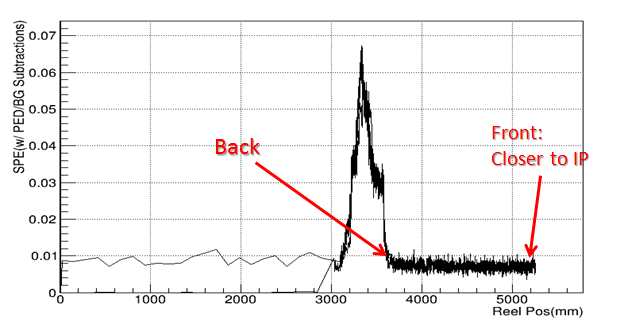
\includegraphics[width=.8\textwidth]{figures/ch_hfcalibration/Signal_ReelPos.png}
        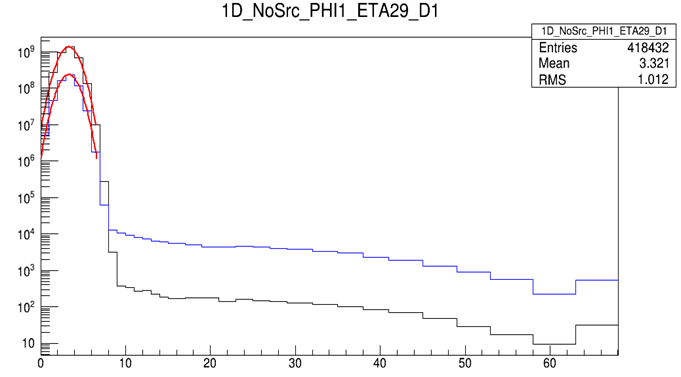
\includegraphics[width=.8\textwidth]{figures/ch_hfcalibration/Signal_Histogram.png}
        \caption
        {(a)Source Signal vs Position (b) 32-bin histogram - A basic object of the read out per a given channel}
        \label{fig:hf_campaigns_histograms}
    \end{center}
\end{figure}

% Run numbers for data collected during this campaign are
% listed in Table~\ref{tab:2013HFM_Runs}.

% \begin{table}[htb] \centering \scalebox{1.10}{
%   \begin{tabular}{|c|c|c|c|c|}
%   \hline
%   Date & Run Number & IPhi & Tubes Sourced & Comments \\
%   \hline
%   \hline
%   23 Oct. & 215590 & 55 & 1A & \\
%   \hline
%   23 Oct. & 215594 & 55 & 1B & \\
%   \hline
%   23 Oct. & 215595 & 55 & 2A-2B & \\
%   \hline
%   23 Oct. & 215596 & 55 & 3A-3B & \\
%   \hline
%   23 Oct. & 215597 & 55 & 4-5 & \\
%   \hline
%   23 Oct. & 215600 & 55 & 6-9 & \\
%   \hline
%   23 Oct. & 215602 & 55 & 10-13 & \\
%   \hline
%   23 Oct. & 215604 & 57 & 14A-15B & \\
%   \hline
%   23 Oct. & 215607 & 57 & 16A-24 & For a few channels, one bin \\
%   &&&& on the tail seems higher in \\
%   &&&& background data than signal data\\
%   \hline
%   24 Oct. & 215631 & 59 & 1A-10 & For a few channels, one bin \\
%   &&&& on the tail seems higher in \\
%   &&&& background than in signal data \\
%   \hline
%   24 Oct. & 215632 & 59 & 1A-10 & Same tubes as Run 215631; one \\
%   &&&& bin on the tail seems higher in \\
%   &&&& background data than signal data \\
%   \hline
%   24 Oct. & 215659 & 59-61 & 11-24 & \\
%   \hline
%   24 Oct. & 215637 & 63 & 1A-13 & \\
%   \hline
%   24 Oct. & 215649 & 65 & 14A-24 & \\
%   \hline
%   25 Oct. & 215689 & 67 & 1A-3B & \\
%   \hline
%   25 Oct. & 215690 & 67 & 4-7 & \\
%   \hline
%   25 Oct. & 215699 & 67 & 8-13 & \\
%           &        & 71 & 14A-15B & \\
%   \hline
%   25 Oct. & 215704 & 69 & 14A-15B & \\
%   \hline
%   25 Oct. & 215706 & 69 & 16A-24 & \\
%   \hline
%   25 Oct. & 215709 & 71 & 1A-13 & \\
%   \hline
%   25 Oct. & 215716 & 1 & 16A-24 & Tubes 14A-15B already \\
%   &&&& sourced in Run 215699 \\
%   \hline
%   25 Oct. & 215719 & 3 & 1A-13 & \\
%   \hline
%   25 Oct. & 215721 & 5 & 14A-24 & \\
%   \hline
%   26 Oct. & 215736 & 7 & 1A-7 & \\
%   \hline
%   26 Oct. & 215738 & 7-9 & 8-15B & \\
%   \hline
%   26 Oct. & 215739 & 9 & 16A-24 & \\
%   \hline
%   26 Oct. & 215741 & 11 & 1A-12B & \\
%   \hline
%   26 Oct. & 215746 & 11-13 & 13-24 & \\
%   \hline
%   27 Oct. & 215748 & 15 & 1A-13 & \\
%   \hline
%   27 Oct. & 215749 & 17 & 14A-24 & \\
%   \hline
%   \end{tabular}}
%   \caption{List of 1TS OV1 runs taken for radioactive source data in HF- during the 2013
%   campaign, with the date data was recorded, run number, $\phi$ index (IPhi) sourced, source
%   tubes sourced, and any related comments concerning data quality.}
%   \label{tab:2013HFM_Runs}
% \end{table}

\subsection{2014 HF+ Campaign}
All four quadrants of HF+ were exposed to the radioactive source on 22 - 27 April
2014, during which the activity of the source was 67.56 $\pm$ 0.18 \unit{MBq}.
At this stage of HCAL upgrades, the new PMTs were installed and functional.
All four quadrants were sourced using the 1 TS firmware at OV1. In addition quadrants 1 and 4, also referred to as the near side of HF+ containing wedges
1-9, were sourced with 2 TS firmware at OV1+100. In the histogramming mode, the
absorber's response charge is represented across 32 bins, but for this campaign
the overflow bin could be included in the analysis because previous issues with
firmware error codes was rectified to exclude any nonphysical entries from the
32 bins. Also, during this campaign, the radioactive source was extended and
retracted into and out of the source tubes without being held stationary at any
point - this procedure differs from that used during the 2013 HF- campaign.


% Run numbers for data collected during this campaign are listed in
% Table~\ref{tab:2014HFP_Runs_1TSOV1} and Table~\ref{tab:2014HFP_Runs_2TSOV1p100}.
% Table~\ref{tab:2014HFP_Errors} lists channel and source tube swaps. A channel swap occurs when two
% QIE connections are swapped, and a source tube swap occurs when the source driver
% mistakes two source tubes by extending the source wire in the wrong tube.

% \begin{table}[htb] \centering \scalebox{1.10}{
%   \begin{tabular}{|c|c|c|c|c|}
%   \hline
%   Date & Run Number & IPhi & Tubes Sourced & Comments \\
%   \hline
%   \hline
%   22 Apr. & 221486 & 19-21 & 1A-24 & \\
%   \hline
%   22 Apr. & 221495 & 19-21 & 1A-24 & \\
%   \hline
%   23 Apr. & 221509 & 23-25 & 1A-24 & \\
%   \hline
%   23 Apr. & 221514 & 27-29 & 1A-24 & Run started after readout \\ &&&& change \\
%   \hline
%   23 Apr. & 221518 & 31-33 & 1A-24 & \\
%   \hline
%   23 Apr. & 221520 & 35-37 & 1A-24 & Run did not finish \\ &&&& with 'Run Over' status \\
%   \hline
%   23 Apr. & 221521 & 39-41 & 1A-24 & \\
%   \hline
%   24 Apr. & 221524 & 43-45 & 1A-24 & \\
%   \hline
%   24 Apr. & 221528 & 47-49 & 1A-24 & \\
%   \hline
%   24 Apr. & 221532 & 51-53 & 1A-24 & Run started after readout \\ &&&& change \\
%   \hline
%   24 Apr. & 221539 & 55-57 & 1A-24 & \\
%   \hline
%   24 Apr. & 221545 & 59-61 & 1A-24 & \\
%   \hline
%   24 Apr. & 221546 & 63-65 & 1A-24 & \\
%   \hline
%   24 Apr. & 221552 & 67-69 & 1A-24 & \\
%   \hline
%   25 Apr. & 221557 & 71, 1 & 1A-24 & Run file did not close \\ &&&& properly \\
%   \hline
%   25 Apr. & 221561 & 3-5 & 1A-24 & \\
%   \hline
%   25 Apr. & 221564 & 7-9 & 1A-24 & \\
%   \hline
%   25 Apr. & 221566 & 11-13 & 1A-24 & \\
%   \hline
%   25 Apr. & 221567 & 15-17 & 1A-24 & \\
%   \hline
%   \end{tabular}}
%   \caption{List of 1TS OV1 runs taken for radioactive source data in HF+ during the 2014
%   campaign, with the date data was recorded, run number, $\phi$ index (IPhi) sourced, source
%   tubes sourced, and any related comments concerning data quality.}
%   \label{tab:2014HFP_Runs_1TSOV1}
% \end{table}

% \begin{table}[htb] \centering \scalebox{1.10}{
%   \begin{tabular}{|c|c|c|c|c|}
%   \hline
%   Date & Run Number & IPhi & Tubes Sourced & Comments \\
%   \hline
%   \hline
%   23 Apr. & 221502 & 19-21 & 1A-24 & \\
%   \hline
%   25 Apr. & 221584 & 15-17 & 1A-24 & \\
%   \hline
%   26 Apr. & 221589 & 11-13 & 1A-24 & \\
%           & 221594 &       &       & \\
%   \hline
%   26 Apr. & 221595 & 7-9 & 1A-24 & \\
%   \hline
%   26 Apr. & 221597 & 3-5 & 1A-24 & \\
%   \hline
%   26 Apr. & 221598 & 71, 1 & 1A-24 & \\
%   \hline
%   26 Apr. & 221599 & 67-69 & 1A-24 & \\
%   \hline
%   26 Apr. & 221602 & 63-65 & 1A-24 & \\
%   \hline
%   27 Apr. & 221608 & 59-61 & 1A-24 & \\
%   \hline
%   27 Apr. & 221609 & 55-57 & 1A-24 & \\
%   \hline
%   \end{tabular}}
%   \caption{List of 2TS OV1+100 runs taken for radioactive source data in HF+ during the 2014
%   campaign, with the date data was recorded, run number, $\phi$ index (IPhi) sourced, source
%   tubes sourced, and any related comments concerning data quality.}
%   \label{tab:2014HFP_Runs_2TSOV1p100}
% \end{table}

% \begin{table}[htb] \centering \scalebox{1.10}{
%   \begin{tabular}{|c|c|c|c|}
%   \hline
%   IEta & IPhi & Channel & Reason \\
%   \hline
%   \hline
%   57 & 29 & EM & Channel Swap \\
%   57 & 30 & EM & Channel Swap \\
%   57 & 31 & EM & Channel Swap \\
%   57 & 32 & EM & Channel Swap \\
%   57 & 33 & EM & Channel Swap \\
%   57 & 34 & EM & Channel Swap \\
%   61 & 35 & EM & Channel Swap \\
%   61 & 36 & EM & Channel Swap \\
%   61 & 37 & EM & Channel Swap \\
%   61 & 38 & EM & Channel Swap \\
%   61 & 39 & EM & Channel Swap \\
%   59 & 40 & EM & Channel Swap \\
%   53 & 29 & H & Channel Swap \\
%   53 & 30 & H & Channel Swap \\
%   53 & 31 & H & Channel Swap \\
%   53 & 32 & H & Channel Swap \\
%   53 & 33 & H & Channel Swap \\
%   53 & 34 & H & Channel Swap \\
%   57 & 35 & H & Channel Swap \\
%   57 & 36 & H & Channel Swap \\
%   57 & 37 & H & Channel Swap \\
%   57 & 38 & H & Channel Swap \\
%   57 & 39 & H & Channel Swap \\
%   55 & 40 & H & Channel Swap \\
%   25 & 35 & H & Channel Swap \\
%   25 & 36 & H & Channel Swap \\
%   25 & 37 & H & Channel Swap \\
%   25 & 38 & H & Channel Swap \\
%   25 & 39 & H & Channel Swap \\
%   23 & 40 & H & Channel Swap \\
%   \hline
%   23 & 34 & EM & Tube Swap \\
%   23 & 35 & EM & Tube Swap \\
%   23 & 34 & H & Tube Swap \\
%   23 & 35 & H & Tube Swap \\
%   \hline
%   \end{tabular}}
%   \caption{$\eta$ index, $\phi$ index, channel type, and reason for any
%   error in data collected during the 2014 HF+ source campaign.}
%   \label{tab:2014HFP_Errors}
% \end{table}

\subsection{2014 HF- Campaign}
All four quadrants of HF- were exposed to the radioactive source on 1 - 11 July
2014, during which the activity of the source was 65.81 $\pm$ 0.21 \unit{MBq}.
As with HF+, the new PMTs were installed and functional in HF- by this time.
All four quadrants were sourced using the 1 TS and 2 TS firmware, separately, at
OV1 and OV1+100, respectively. For this campaign, the overflow bin could be
included in the analysis because previous issues with firmware error codes were
rectified to exclude any nonphysical entries from the 32 bins. Also, during
this campaign, the radioactive source was extended and retracted into and out
of the source tubes without being held stationary at any point - this
procedure differs from that used during the 2013 HF- campaign.

% Run numbers for data collected during this campaign are listed in
% Table~\ref{tab:2014HFM_Runs_1TSOV1} and Table~\ref{tab:2014HFM_Runs_2TSOV1p100}.
% Table~\ref{tab:2014HFM_Errors} lists channel and source tube swaps, as well as source driver errors.
% A source driver error occurs when the radioactive source did not fully penetrate
% the intended absorber.

% \begin{table}[htb] \centering \scalebox{1.10}{
%   \begin{tabular}{|c|c|c|c|c|}
%   \hline
%   Date & Run Number & IPhi & Tubes Sourced & Comments \\
%   \hline
%   \hline
%   8 July & 222804 & 19 & 1A-13 & \\
%   \hline
%   8 July & 222811 & 21 & 14A-24 & \\
%   \hline
%   8 July & 222817 & 23 & 1A-13 & \\
%   \hline
%   8 July & 222822 & 25 & 14A-24 & \\
%   \hline
%   9 July & 222828 & 27 & 1A-13 & \\
%   \hline
%   9 July & 222831 & 29 & 14A-24 & \\
%   \hline
%   9 July & 222837 & 31 & 1A-13 & \\
%   \hline
%   9 July & 222843 & 33 & 14A-24 & \\
%   \hline
%   9 July & 222845 & 35 & 1A-13 & \\
%   \hline
%   9 July & 222846 & 37 & 14A-24 & \\
%   \hline
%   9 July & 222847 & 39 & 1A-13 & \\
%   \hline
%   9 July & 222848 & 41 & 14A-24 & \\
%   \hline
%   9 July & 222849 & 43 & 1A-13 & \\
%   \hline
%   9 July & 222853 & 45 & 14A-24 & \\
%   \hline
%   9 July & 222854 & 47 & 1A-13 & \\
%   \hline
%   9 July & 222855 & 49 & 14A-24 & \\
%   \hline
%   9 July & 222856 & 51 & 1A-13 & \\
%   \hline
%   9 July & 222859 & 53 & 14A-24 & \\
%   \hline
%   10 July & 222862 & 55 & 1A-13 & \\
%   \hline
%   10 July & 222863 & 57 & 14A-24 & \\
%   \hline
%   10 July & 222864 & 59 & 1A-13 & \\
%   \hline
%   10 July & 222870 & 61 & 14A-24 & \\
%   \hline
%   10 July & 222873 & 63 & 1A-13 & \\
%   \hline
%   10 July & 222879 & 65 & 14A-24 & \\
%   \hline
%   10 July & 222886 & 67 & 1A-13 & \\
%   \hline
%   10 July & 222888 & 69 & 14A-24 & \\
%   \hline
%   10 July & 222892 & 71 & 1A-13 & \\
%   \hline
%   11 July & 222906 & 1 & 14A-24 & \\
%   \hline
%   11 July & 222907 & 3 & 1A-13 & \\
%   \hline
%   11 July & 222910 & 5 & 14A-24 & \\
%   \hline
%   11 July & 222913 & 7 & 1A-13 & \\
%   \hline
%   11 July & 222918 & 9 & 14A-24 & \\
%   \hline
%   11 July & 222922 & 11 & 1A-13 & \\
%   \hline
%   11 July & 222923 & 13 & 14A-24 & \\
%   \hline
%   11 July & 222930 & 15 & 1A-13 & \\
%   \hline
%   11 July & 222935 & 17 & 14A-24 & \\
%   \hline
%   \end{tabular}}
%   \caption{List of 1TS OV1 runs taken for radioactive source data in HF- during the 2014
%   campaign, with the date data was recorded, run number, $\phi$ index (IPhi) sourced, source
%   tubes sourced, and any related comments concerning data quality.}
%   \label{tab:2014HFM_Runs_1TSOV1}
% \end{table}

% \begin{table}[htb] \centering \scalebox{1.10}{
%   \begin{tabular}{|c|c|c|c|c|}
%   \hline
%   Date & Run Number & IPhi & Tubes Sourced & Comments \\
%   \hline
%   \hline
%   1 July & 222328 & 55 & 1A-3B & Only 3 tubes were sourced\\
%   \hline
%   1 July & 222336 & 55 & 4-13 & IEta = 32-41 \\
%   \hline
%   1 July & 222338 & 57 & 14A-24 & \\
%   \hline
%   2 July & 222364 & 59 & 1A-13 & \\
%   \hline
%   2 July & 222365 & 61 & 14A-24 & \\
%   \hline
%   2 July & 222375 & 63 & 1A-13 & \\
%   \hline
%   2 July & 222387 & 65 & 14A-24 & \\
%   \hline
%   2 July & 222411 & 67 & 1A-13 & \\
%   \hline
%   2 July & 222423 & 69 & 14A-24 & \\
%   \hline
%   2 July & 222432 & 71 & 1A-13 & \\
%   \hline
%   2 July & 222481 & 1 & 14A-24 & \\
%   \hline
%   3 July & 222501 & 3 & 1A-13 & \\
%   \hline
%   3 July & 222502 & 5 & 14A-24 & \\
%   \hline
%   3 July & 222507 & 7 & 1A-13 & \\
%   \hline
%   3 July & 222532 & 9 & 14A-24 & \\
%   \hline
%   3 July & 222541 & 11 & 1A-13 & \\
%   \hline
%   3 July & 222574 & 13 & 14A-24 & \\
%   \hline
%   3 July & 222598 & 15 & 1A-13 & \\
%   \hline
%   3 July & 222609 & 17 & 14A-24 & \\
%   \hline
%   4 July & 222681 & 19 & 1A-13 & \\
%   \hline
%   4 July & 222703 & 21 & 14A-24 & \\
%   \hline
%   4 July & 222710 & 23 & 1A-13 & \\
%   \hline
%   4 July & 222719 & 25 & 14A-24 & \\
%   \hline
%   5 July & 222726 & 27 & 1A-13 & \\
%   \hline
%   5 July & 222727 & 29 & 14A-24 & \\
%   \hline
%   5 July & 222728 & 31 & 1A-13 & \\
%   \hline
%   5 July & 222729 & 33 & 14A-24 & \\
%   \hline
%   5 July & 222731 & 35 & 1A-13 & \\
%   \hline
%   5 July & 222739 & 37 & 14A-24 & \\
%   \hline
%   5 July & 222740 & 39 & 1A-13 & \\
%   \hline
%   5 July & 222741 & 41 & 14A-24 & \\
%   \hline
%   5 July & 222742 & 43 & 1A-13 & \\
%   \hline
%   8 July & 222776 & 45 & 14A-24 & \\
%   \hline
%   8 July & 222784 & 47 & 1A-13 & \\
%   \hline
%   8 July & 222786 & 49 & 14A-24 & \\
%   \hline
%   8 July & 222789 & 51 & 1A-3B & Driver stopped at Tube 3B \\
%   \hline
%   8 July & 222797 & 51 & 4-13 & \\
%   \hline
%   8 July & 222800 & 53 & 14A-24 & \\
%   \hline
%   \end{tabular}}
%   \caption{List of 2TS OV1+100 runs taken for radioactive source data in HF- during the 2014
%   campaign, with the date data was recorded, run number, $\phi$ index (IPhi) sourced, source
%   tubes sourced, and any related comments concerning data quality.}
%   \label{tab:2014HFM_Runs_2TSOV1p100}
% \end{table}

% \begin{table}[htb] \centering \scalebox{1.10}{
%   \begin{tabular}{|c|c|c|c|}
%   \hline
%   IEta & IPhi & Channel & Reason \\
%   \hline
%   \hline
%   55 & 41 & EM & Channel Swap \\
%   57 & 39 & EM & Channel Swap \\
%   57 & 38 & EM & Channel Swap \\
%   57 & 37 & EM & Channel Swap \\
%   57 & 36 & EM & Channel Swap \\
%   57 & 35 & EM & Channel Swap \\
%   59 & 35 & EM & Channel Swap \\
%   59 & 36 & EM & Channel Swap \\
%   59 & 37 & EM & Channel Swap \\
%   59 & 38 & EM & Channel Swap \\
%   59 & 39 & EM & Channel Swap \\
%   59 & 40 & EM & Channel Swap \\
%   11 & 35 & H & Channel Swap \\
%   11 & 36 & H & Channel Swap \\
%   11 & 37 & H & Channel Swap \\
%   11 & 38 & H & Channel Swap \\
%   11 & 39 & H & Channel Swap \\
%   11 & 40 & H & Channel Swap \\
%   67 & 35 & H & Channel Swap \\
%   67 & 36 & H & Channel Swap \\
%   67 & 37 & H & Channel Swap \\
%   67 & 38 & H & Channel Swap \\
%   67 & 39 & H & Channel Swap \\
%   67 & 40 & H & Channel Swap \\
%   \hline
%   1 & 36 & EM & Tube Swap \\
%   1 & 37 & EM & Tube Swap \\
%   1 & 36 & H & Tube Swap \\
%   1 & 37 & H & Tube Swap \\
%   53 & 29 & EM & Tube Swap \\
%   53 & 30 & EM & Tube Swap \\
%   53 & 29 & H & Tube Swap \\
%   53 & 30 & H & Tube Swap \\
%   \hline
%   51 & 31 & EM & Source did not penetrate during 2TS OV1+100 data \\
%   51 & 31 & H & Source did not penetrate during 2TS OV1+100 data \\
%   21 & 29 & EM & Source did not penetrate during 1TS OV1 data \\
%   21 & 29 & H & Source did not penetrate during 1TS OV1 data \\
%   21 & 38 & EM & Source did not penetrate during 1TS OV1 data \\
%   21 & 38 & H & Source did not penetrate during 1TS OV1 data \\
%   43 & 41 & EM & Source did not penetrate during 1TS OV1 data \\
%   43 & 41 & H & Source did not penetrate during 1TS OV1 data \\
%   \hline
%   \end{tabular}}
%   \caption{$\eta$ index, $\phi$ index, channel type, and reason for any
%   error in data collected during the 2014 HF- source campaign.}
%   \label{tab:2014HFM_Errors}
% \end{table}

\section{Analysis Procedure}
The main objective of the HF sourcing analysis is to transfer the HF energy
calibration used in Run I to a new hardware to be used during Run II. More
specifically, it is to compute calibration coefficients (so called "HF
Gains", not to be confused with PMT gains), validate them, and upload the
results to the offline database for further use. All the data files
collected during these campaigns are stored on disk at CERN in the EOS
storage system.

The general content of the data files is reduced to include pertenant
information for calibration, such as the indexes of each channel powered
during the campaign, a two-dimensional array containing each channel's
output signal and capacitor ID (CapID), the name of the source tube being
sourced during any given event, the position of the radioactive source
with respect to the source driver, etc. The reduced data file is still
substantially large given that many wedges were connected to power during
each campaign, each providing output signals for its 24 towers at two
channels per tower (EM or H).

The output (EM and H channels) from the tower containing the
radioactive source are considered signal data, while the background data
is collected for each tower while the radioactive source is sufficiently
far away. To gaurantee that the radioactive source is sufficeintly distant
from a given tower measuring background data, we require the following of
each tower's $\eta$ index (IEta) for a wedge half with a given $\phi$
index (IPhi):
\begin{center}
   \begin{eqnarray}
      \label{eq:Tower_Cuts}
      \textrm{Source in IEta = 29: Record Background for IEta $\ge$ 34,} \\
      \textrm{Source in IEta = 39: Record Background for IEta $<$ 34.} \nonumber
   \end{eqnarray}
\end{center}

Therefore, for a given channel within a given tower and wedge, we collect
separately the signal and background data based on the location of the
radioactive source described above. Provided that histograms for each channel
are being read out by the DAQ at a rate of every four events, and each event
contains all four capacitors' histograms for each QIE, then we loop over all
events recorded for a given channel and sum together all four capacitors'
histograms. To eliminate extraneous data resulting from energy deposition
in the optical fiber bundles as the radioactive source has yet to fully
penetrate the absorber, we restrict the loop over events when source is positioned strictly inside of the calorimeter: [start + 300 mm, end - 300 mm],
where start and end are the distances from the source driver at
which the given source tube begins and ends within the absorber, respectively.
The reason we also exclude data when the radioactive source nears the Tube End
position is due to extraneous data resulting from some optical fibers extending
beyond the length of the absorber. This tail end cut also helps in unifying
signal data definitions between the EM and H channels, given that the H fibers
are shorter in length than the EM fibers.

In combining the histograms from all four capacitors within an event, we can
then study the newly constructed total histogram as a function of reel position
of the radioactive source within the absorber - this ability is crucial for
radiation damage studies within the HF calorimeters. However, for the intent of
calibrating the new PMTs installed for Run II, we choose to focus on comparing
the total energy deposition recorded within a given tower with the expected
energy deposition provided from the radioactive source. Therefore, we constuct
a 32 bin histogram, with similar ADC charge bin ranges as provided by the
firmware, that stores the overall sum of all events' 4-capacitor histograms
according to the following:

\begin{center}
   \begin{equation}
      \label{eq:Histo_Sum}
      N_j = \sum\limits_{i=l}^m \sum\limits_{CapID=1}^4 n_j
   \end{equation}
\end{center}

where $N_j$ and $n_j$ are the content of the $j^{th}$ bin of their respective
histograms, and $i$ is the event with $l$ and $m$ restricted according to
Eq.~\ref{eq:Reel_Cuts}.

We define the mean ADC charge separately for signal and background data of a
particular tower by averaging over the bins of the total histogram from all
events,

\begin{center}
   \begin{eqnarray}
      \label{eq:Histo_Avg}
      \langle{Q}\rangle = (\frac{1}{N} \sum\limits_{j=1}^{31} N_{j}q_{j}) - P, \\
      N = \sum\limits_{j=1}^{31} N_j \nonumber
   \end{eqnarray}
\end{center}

where $\langle{Q}\rangle$ is the mean ADC charge for the total histogram,
$N$ is the total number of entries within the bin range [1,31], $q_j$ is
the central ADC charge for the $j^{th}$ bin, and $P$ is the Gaussian mean of
the pedestal region. All sourcing histograms have a clear feature of a pedestal
peak. That is due to the fact that there is no actual trigger during
histogramming mode. Every TS data gets recorded. Therefore the number of events
that fall under the pedestal is several orders of magnitude larger than in the
beyond pedestal region, and the $\mu$ and $\sigma$ of the pedestal are dominated
by histogram's mean and width. We compute $P$ by fitting the histogram
within the pedestal region [$\mu$ - 4$\sigma$, $\mu$ + 4$\sigma$]
(if lower bound falls below 0, take 0 as the min value) with a Gaussian function
and extracting the function's mean. This act of fitting the pedestal
and removing it from the mean ADC charge for signal and background histograms
separately performs a dynamic treatment of this
background, as the pedestal mean typically shifts, or fluctuates, from event
to event, but between background and source histgorams (which ideally isn't the case).

To determine the charge deposition for a given channel of a tower,
${\langle{Q}\rangle}_c$~, we then must subtract out the background mean ADC
charge, ${\langle{Q}\rangle}^{(b)}_{c}$, from the signal yield,
${\langle{Q}\rangle}^{(s)}_{c}$, as follows:

\begin{center}
   \begin{equation}
      \label{eq:Sig_Min_Bkg}
      {\langle{Q}\rangle}_{c} = {\langle{Q}\rangle}^{(s)}_{c} - {\langle{Q}\rangle}^{(b)}_{c}.
   \end{equation}
\end{center}

To account for energy leakage, due to the restraints on geometric
containment of the radiated energy from the radioactive source within the tower,
we must apply the geometric correction factors, $G_c$~, listed in
Table~\ref{tab:hf_description_gcfactors} as follows:

\begin{center}
   \begin{equation}
      \label{eq:Sig_Corr}
      {\langle{Q}\rangle}^{Geom}_{c} = \frac{{\langle{Q}\rangle}_{c}}{G_{c}}\unit{ADC/25ns}.
   \end{equation}
\end{center}

Up to this point, the analysis procedure was identical for both 2013 and 2014
Sourcing Campaigns. However, to proceed further with calibration (calculating the
actual HF Gains), the source energy deposition had to be extracted from 2013 data.

\subsection{Extracting Source Energy Deposition}
The source energy deposition is the amount of energy deposited by the source in
units of GeV/25 ns. The actual source signal is measured (computed) in
ADC/25 ns. Therefore, we need a conversion factor GeV/ADC, which comes from
Run I Conditions. To extract Run I HF Gains and QIE Slopes from the Conditions DataBase (CondDB), we used Run 203777. Since 2013 sourcing was performed with the old PMTs, the
Calibration Coefficients ${CC}^{Run I}_{c}$~ (GeV/ADC) used during Run I were used to convert
the signal measured in ADC/25\unit{ns} into GeV/25\unit{ns}. It is important to point out that in our calculation of energy deposition, we didn't include response corrections. That is because we would like to preserve Run I calibration for PMT gains, when extractin the energy, but not the HF response, which is affected by other corrections accumulated in response corrections.

In Figure~\ref{fig:QIE_Slope}, correlation plots between the inverted Calibration
Coefficients (ADC/GeV) from Run I and Source Signal (ADC/25\unit{ns}) from 2013
Campaign are presented. Here we use a similar strategy to Run I Calibration, when
EM and HAD channels were calibrated separately. Except for some outlier channels,
we observe a good correlation between Signals collected (in 2013) and the Run I
Calibration Constants. Therefore, we can extract Source Energy Deposition:

\begin{center}
	\begin{equation}
		\label{eq:Edep}
		{\langle{E}\rangle}_{c} = {\langle{Q}\rangle}^{Geom}_{c} \times {CC^{Run I}_{c}}.
	\end{equation}
\end{center}


\begin{figure}[htb]
   \begin{center}
      \subfigure[]{
         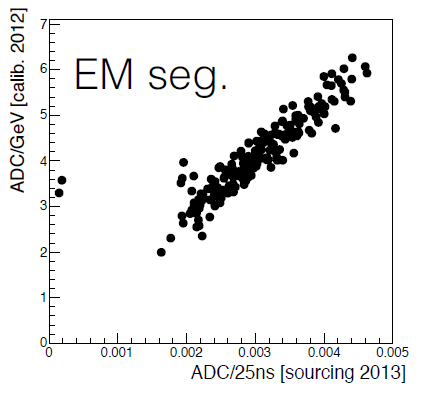
\includegraphics[width=.4\textwidth]{figures/ch_hfcalibration/QIE_Res_EM.png}
      }
      \subfigure[]{
         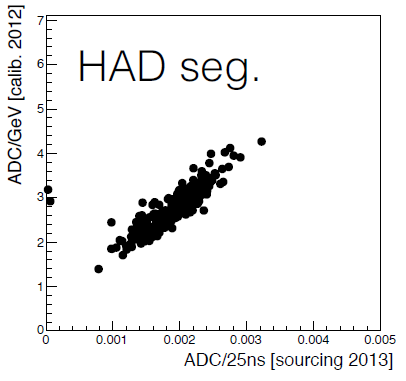
\includegraphics[width=.4\textwidth]{figures/ch_hfcalibration/QIE_Res_H.png}
      }
      \caption{(a) Correlation plot between QIE response, in ADC/GeV, and 2013 HF-
               geometry corrected energy deposition, in ADC/25\unit{ns}, per tower
               for the EM channel.
               (b) Similar correlation is observed for the H channel.}
      \label{fig:QIE_Slope}
   \end{center}
\end{figure}

\subsection{Calculating Calibration Coefficients}
During Run II, HF will be operated at the Operational Voltage 2 (OV2). Since
both 2014 sourcing campaigns were done at voltage settings, OV1 and OV1+100,
different from the one to be used, we have to convert the actual source signals to
the needed voltage, by using gains for the respective voltages. Another factor to
account for is the firmware setting, either 1TS or 2TS. Taking these 2 arguments
into account, we compute a source signal at OV2 in units of ADC/25\unit{ns}:
\begin{center}
	\begin{equation}
		\label{eq:Sig_OV2}
		{\langle{Q}\rangle}^{Geom,OV2}_{c} = \frac{{\langle{Q}\rangle}^{Geom}_{c}}{nTS} \times \frac{{GAIN}^{OV2}}{{GAIN}^{OV1,OV1+100}}.
	\end{equation}
\end{center}
Finally, we compute the actual Calibration Coefficients (HF Gains) ${CC}^{Run II}_{c}$:
\begin{center}
	\begin{equation}
		\label{eq:HF_Gains}
		{CC}^{Run II}_{c} = \tau \times \frac{{\langle{E}\rangle}^{2013}}{{\langle{Q}\rangle}^{Geom, OV2}_{c}}.
	\end{equation}
\end{center}
where $\tau$ is the source radioactivity correction factor, which accounts for exponential source activity decrease. We take 2013 sourcing date as the starting point and compute the decrease for April and July 2014 with respect to that date.

\section{Results and Discussion}
\subsection{2013 Results}
As it has already been pointed out, outlier channels from Figure~\ref{fig:QIE_Slope} have been excluded.
Moreover, to achieve a result for the average energy deposition per channel type,
EM or H, from the radioactive source, we only considered data from towers with
IEta $<$ 35 to minimize the effects of radiation damage of HF fibers at higher $\eta$ towers, shown in Figure~\ref{fig:PMT_Drift}.
\begin{figure}[htb]
   \begin{center}
      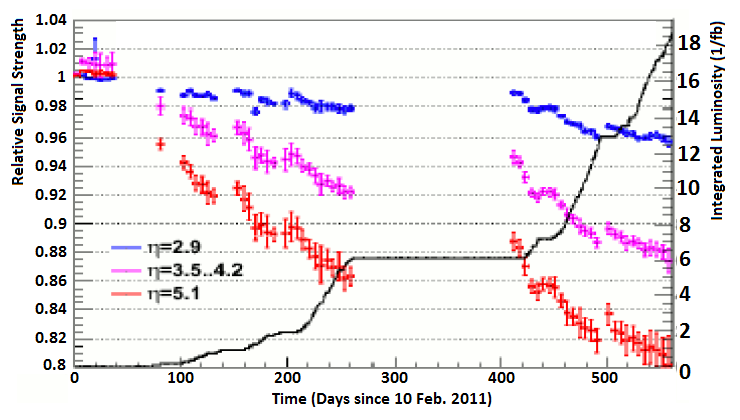
\includegraphics[width=.9\textwidth]{figures/ch_hfcalibration/PMT_Drift.png}
      \caption{R7525 PMT relative signal strength with respect to 10 Feb. 2011 as a
      function of time since that date, for various $\eta$ locations. The solid
      black curve represents the integrated luminosity within CMS over the same
      time period}
      \label{fig:PMT_Drift}
   \end{center}
\end{figure}

Figure~\ref{fig:HFM_2013_Res} shows the results from 2013 when only the near side
of HF- was sourced, nine wedges, and only the towers below IEta = 35 are
considered, eight towers per wedge. The average energy deposition extracted from
2013 sourcing campaign, for EM and H channels separately, is 744.6 $\pm$ 6.3 keV and 706.8 $\pm$ 7.7 keV per time slice, respectively. There is a 5\% difference observed between the EM and HAD channels, while their
respective precision is kept within 1 \% each.
\begin{figure}[htb]
   \begin{center}
      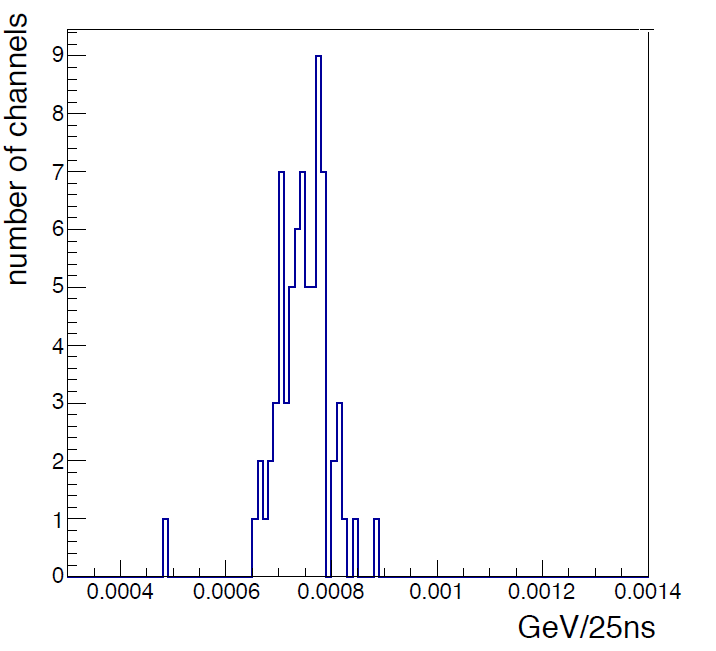
\includegraphics[width=.45\textwidth]{figures/ch_hfcalibration/HFM_2013_Res_EM.png}
      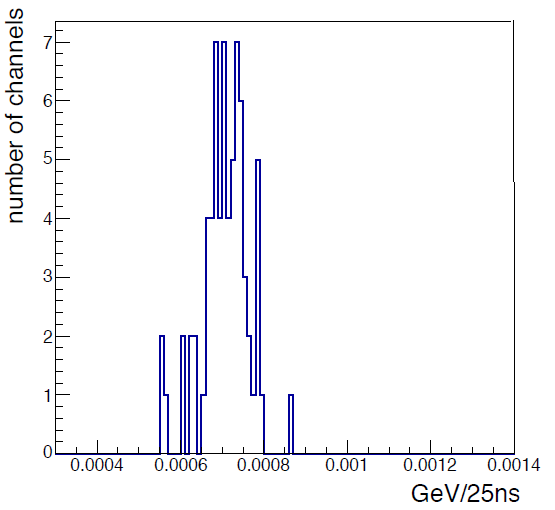
\includegraphics[width=.45\textwidth]{figures/ch_hfcalibration/HFM_2013_Res_H.png}
      \caption{(a) EM Energy deposition for each tower below IEta = 35. (b) H Energy deposition for the same towers}
      \label{fig:HFM_2013_Res}
   \end{center}
\end{figure}

\subsection{2014 Results}
The source signals, ${\langle{Q}\rangle}^{Geom}_{c}$, for HF+ and HF- for 2014 data with new PMTs, corrected for geometry (geometry containment factor), firmware used (1 TS or 2 TS), Operating Voltage to be used (converting to OV2 from either OV1 or OV1+100), are calculated using Equation~\ref{eq:Sig_OV2} and are presented in Figure~\ref{fig:Signal_@OV2_TT0_withoutOF_FORDN}.
\begin{figure}[htb]
	\begin{center}
		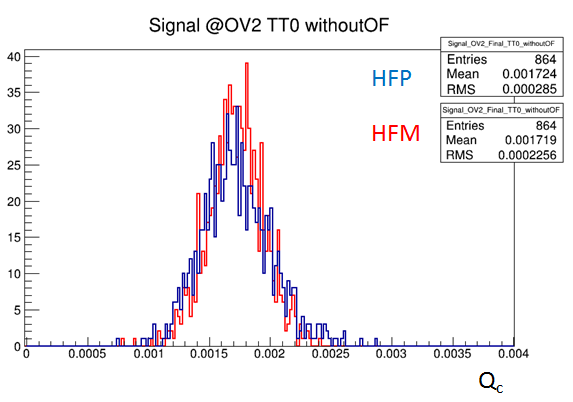
\includegraphics[width=.6\textwidth]{figures/ch_hfcalibration/Signal_@OV2_TT0_withoutOF_FORDN.png}
		\caption{Actual Signal from the Source recorded by the PMT at OV2 (Operational Voltage 2)}
		\label{fig:Signal_@OV2_TT0_withoutOF_FORDN}
	\end{center}
\end{figure}

The HF Gains, ${CC}^{Run II}_{c}$ in units of GeV/ADC, for HF+ and HF- are
computed using Equation~\ref{eq:HF_Gains} and are presented in Figure~\ref{fig:ADC2GeV_OV2_TT0_withoutOF_FORDN}. In Equation~\ref{eq:HF_Gains}, if $c$ is a EM channel from a given tower, then use the EM result from 2013, and similar logic applies for the H channel counterparts.
\begin{figure}[!h]
	\begin{center}
		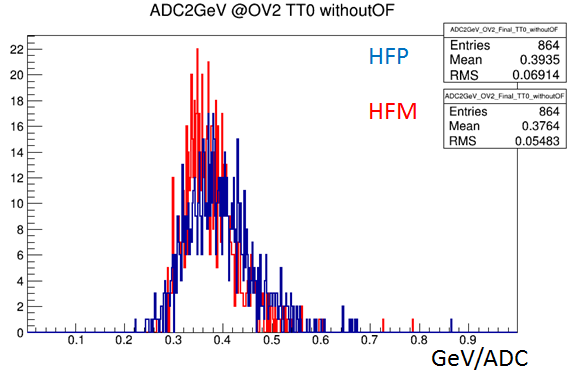
\includegraphics[width=.6\textwidth]{figures/ch_hfcalibration/ADC2GeV_OV2_TT0_withoutOF_FORDN.png}
		\caption{Distribution of Calibration Coefficients (HF Gains)}
		\label{fig:ADC2GeV_OV2_TT0_withoutOF_FORDN}
	\end{center}
\end{figure}

To account for the differences in Operating Voltages for Sourcing vs Run II Physics campaign, the PMT Gain Ratios were applied as Conversion Factors, distributions of which can be found in Figure~\ref{fig:PMT_Gains}
\begin{figure}[!h]
	\begin{center}
		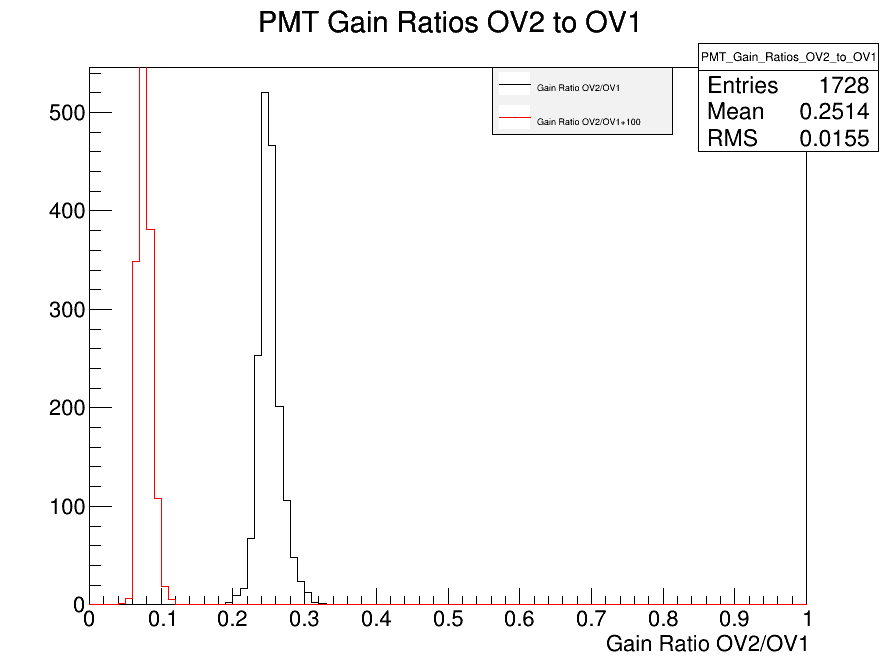
\includegraphics[width=.5\textwidth]{figures/ch_hfcalibration/GainRatios.png}
		\caption
		{Black - Ratio of PMT Gains for OV2/OV1. Red - Ratio of PMT Gains for OV2/OV1+100}
		\label{fig:PMT_Gains}
	\end{center}
\end{figure}

% \subsection{HF Gains and CondDB Submission}
% To finalize the HF Source Calibration, we had to upload the computed calibration
% coefficients, ${CC}^{Run II}_{c}$, into the Conditions DataBase (CondDB).
% However, up until now, the units we used to present them were GeV/ADC, whereas
% for submission it is required to provide calibration coefficients in GeV/fC.

% \begin{figure}[htb]
% 	\begin{center}
% 		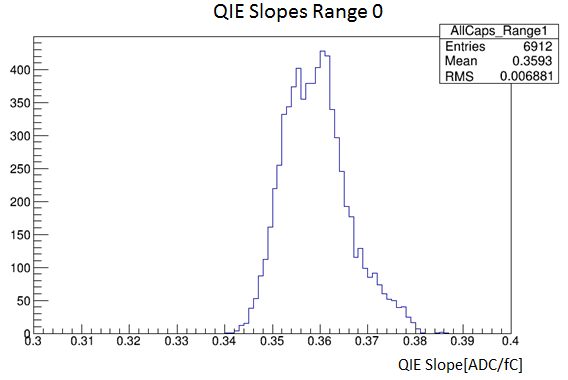
\includegraphics[width=.5\textwidth]{figures/ch_hfcalibration/QIE_Slopes_Range0.png}
% 		\caption{Distribution of Range 0 QIE Slopes}
% 		\label{fig:QIESlopes}
% 	\end{center}
% \end{figure}

% Therefore, we first extracted the ADC to fC conversion factors from the CondDB,
% which are also called "QIE Slopes". As we have only been using Range 0 for
% calibration purposes, they are the only ones of interest to us. At the time when
% the actual analysis was performed, the half of the QIE Slopes were still mixed
% up, as a consequence we averaged out all the slopes and used the mean for
% converting our GeV/ADC to GeV/fC. In the Figure~\ref{fig:QIESlopes}, the
% distribution of Range 0 QIE Slopes is presented. The obtained mean of 0.3593
% (ADC/fC), as it was already pointed out, has been used to calculate the "final"
% calibration coefficients in units of GeV/fC, which are presented in the
% Figure().
% Using the mean of Range 0 QIE Slopes adds an additional
% uncertainty of 2\%, which can be deduced from the spread in the distribution of
% QIE Slopes in the Figure~\ref{fig:QIESlopes}.


\section{Systematics Evaluation}
\subsection{1TS vs. 2TS}
The very first systematic study we did was to compare the results between 2
firmware configurations. All of HFM towers and half of HFP were sourced twice,
using either 1TS (with Operating Voltage 1) or 2TS (using Operating Voltage 2),
which provides us a measure of consistency in computing the calibration
coefficient across different firmware versions and operating voltages.
To compare these 2 modes of operation, we used ${CC}^{Run II}_{c}$ computed for
each sourcing configuration, after applying all the required corrections. The
distributions of ratios (1TS over 2TS) is presented in the Figures~\ref{fig:HF_1TSto2TS}. Comparing 1TS OV1 and 2TS OV1+100 results, the source signals computed need to be corrected for the 25\unit{ns} vs. 50\unit{ns} integration window. After correcting between the firmware gains, the results agree to an order of 1\%.

\begin{figure}[!h]
    \begin{center}
        \subfigure[]
        {
            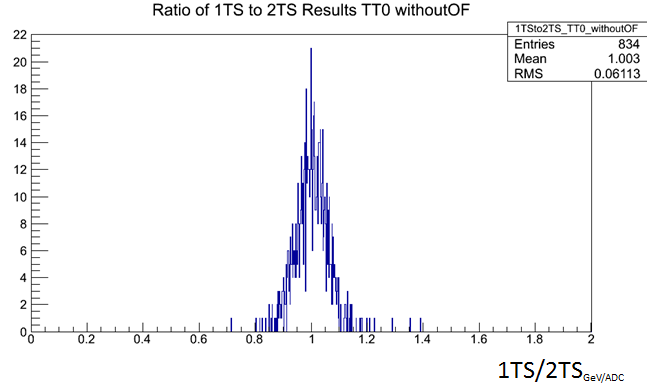
\includegraphics[width=.45\textwidth]{figures/ch_hfcalibration/HFM_1TSto2TS_woOF.png}
        }~
        \subfigure[]
        {
            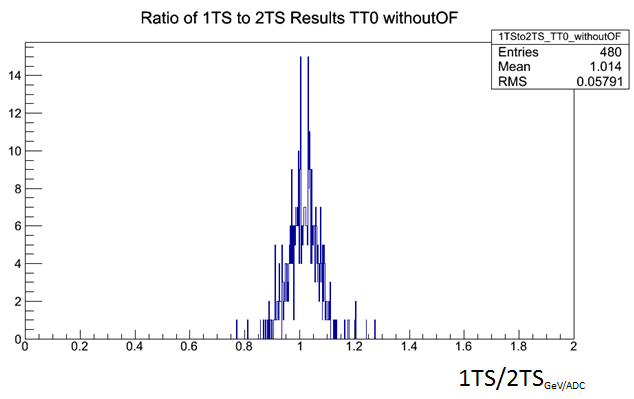
\includegraphics[width=.45\textwidth]{figures/ch_hfcalibration/HFP_1TSto2TS_woOF.png}
        }
        \caption
        {(a) Ratio of 1TS/2TS results for HFM.
         (b) Ratio of 1TS/2TS results for HFP
         For both sides The compared quantity was ${CC}^{Run II}_{c}$}
        \label{fig:HF_1TSto2TS}
    \end{center}
\end{figure}

As observed in the Figures~\ref{fig:HF_1TSto2TS},
1TS and 2TS results match both for HFP (1.4\%) and HFM (0.3\%) on the order of
under 1.5\%, which establishes solid indpendence of calibration coefficients from
the firmware used.

\subsection{Transversal Uniformity: Tubes A vs. Tubes B}
Approximately a quarter of HF wedges contains a second sourcing tube, which
differ in the groove type and as a consequence in the location within a wedge.
By comparing the obtained calibration coefficients using sourcing data from both
tubes, we can extract information on the transversal uniformity (or non-uniformity if you prefer) of the signal
within a wedge. Again, as in the case of 1TS-2TS study, we were comparing the
actual ${CC}^{Run II}_{c}$. The ratios are presented in the Figure~\ref{fig:HF_A2B}. Transversal uniformity between A and B tubes within towers containing them, which is a quarter of the towers within a given wedge, show good agreement between results as well, differing by under 1\%.

\begin{figure}[htb]
    \begin{center}
        \subfigure[]
        {
            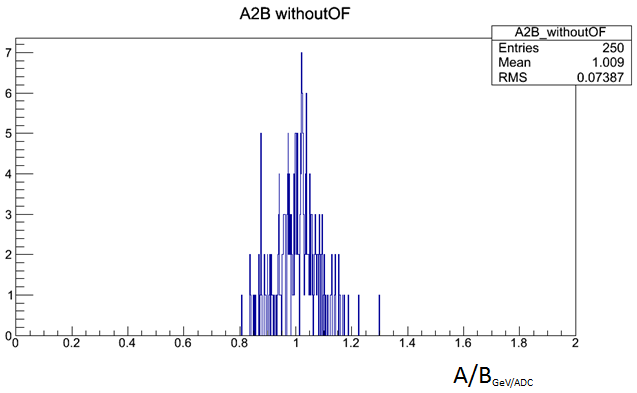
\includegraphics[width=.45\textwidth]{figures/ch_hfcalibration/HFM_A2B_woOF.png}
        }~
        \subfigure[]
        {
            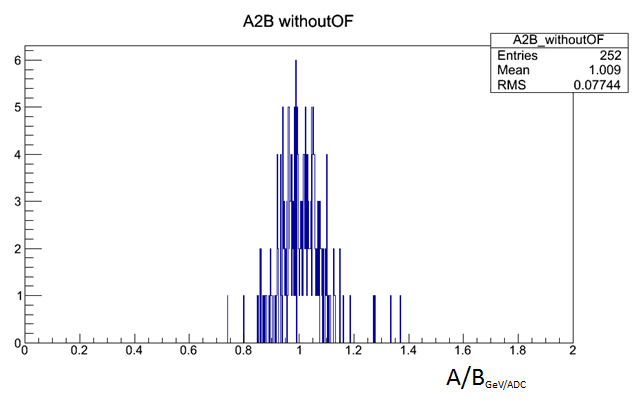
\includegraphics[width=.45\textwidth]{figures/ch_hfcalibration/HFP_A2B_woOF.png}
        }
        \caption
        {(a) Ratio of A/B results for HFM.
         (b) Ratio of A/B results for HFP
         For both sides The compared quantity was ${CC}^{Run II}_{c}$}
        \label{fig:HF_A2B}
    \end{center}
\end{figure}

As observed in the Figure~\ref{fig:HF_A2B}, on average the difference between
signals coming from A and B is on order of 1\%. The channel-to-channel variation
of the ratio is attributed to the Transversal Non-Uniformity of HF Wedges.

\subsection{Overflow Estimation}
Having the overflow bin is the major limitation of the DAQ system and the source of
systematic uncertainty for our analysis. As it was mentioned in the Experimental
Setup Section, both firmware types exhibit this behavior and even though 2TS
has a wider ADC range, the results will not differ dramatically from 1TS, because
differences in operating voltages will balance things out. However, in order to
provide some kind of "Lower Bound" error estimation for our charge measurement,
we separately computed calibration coefficients including the last bin in the
Eq.~\ref{eq:Histo_Avg} and compared them to the ones computed without. The results
for both HFM and HFP are presented in the Figure~\ref{fig:HF_Overflow}. Since we
do not know the actual adc counts in the overflow, when computing charge, we used
the center of the 32nd bin, as it was explained in the Experimental Setup section,
using which does provide us with "Lower Bound" estimation.

\begin{figure}[!h]
    \begin{center}
        \subfigure[]
        {
            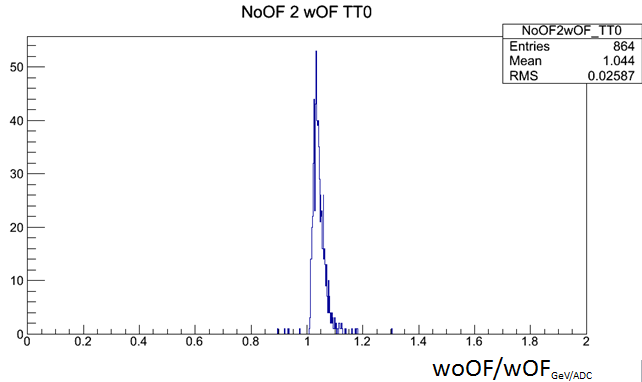
\includegraphics[width=.45\textwidth]{figures/ch_hfcalibration/HFM_NoOF2wOF_gevadc.png}
        }~
        \subfigure[]
        {
            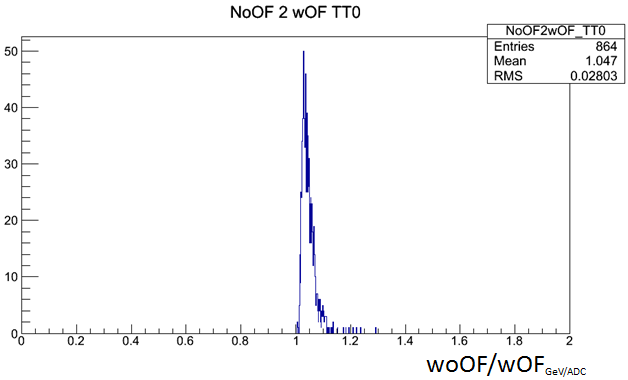
\includegraphics[width=.45\textwidth]{figures/ch_hfcalibration/HFP_NoOF2wOF_gevadc.png}
        }
        \caption
        {(a) Ratio of woOF/wOF results for HFM.
         (b) Ratio of woOF/wOF results for HFP
         For both sides The compared quantity was ${CC}^{Run II}_{c}$.
         Important to note that the ratio appears to be $\geq1$ because the compared quantity isn't a signal, but rather an actual calibration coefficient,
         which contains energy over charge.}
        \label{fig:HF_Overflow}
    \end{center}
\end{figure}

As it can be observed in the Figure~\ref{fig:HF_Overflow}, the calibration
coefficients computed including the overflow bin introduce at least 4.4-4.7\%
difference into the measurement compared to the ${CC}^{Run II}_{c}$ computed
excluding overflow. These 4.4-4.7\% give us a lower bound on the amount of charge
that is approximately "sitting" in the overflow bin compared to the rest of the
ADC range. However, taking into consideration that we subtracted the pedestal
dynamically (inside the sum), we can notice that this is the amount of charge in
the overflow compared to the actual charge deposited by the radioactive source
(meaning that these charges are already pedestal-subtracted, which is very
important, considering that number of events in the pedestal dominate substantially).
Moreover, the actual number of events sitting in the overflow is under 1\% with
respect to the same ADC range. And considering that our integration window is
25\unit{ns} long, it is important to exclude for calibration purposes any
non-promptly originated signals.
It is also important to note that overflow contribution was excluded when analyzing 2013 sourcin campaign, as it didn't contain just overflow charge, but it also any event which was marked as a "hardware failure" went into the overflow bin.

\subsection{Longitudinal Uniformity}
As the radioactive source is moving along the source tube, we are actually able to record the spatial information on the location of the source, which provides us with yet another tool to estimate the uncertainty of our measurements. The general idea is that we defined several regions along the source tube, summed up all the histograms for each region respectively and then extracted the charges and compared them.
\begin{table}[!h] \centering \scalebox{1.10}{
    \begin{tabular}{|c|c|c|}
    \hline
    Region Name & Start & End \\
    \hline
    \hline
    Front(Depth 1 or EM) & tubeEnd-400 & tubeEnd-100 \\
    Front(Depth 2 or HAD) & tubeEnd-700 & tubeEdn-400 \\
    Back & tubeStart+100 & tubeStart+400 \\
    2/3Back & tubeStart & tubeStart+2/3(tubeEnd - tubeStart) \\
    Signal(EM and HAD) & tubeStart+300 & tubeEnd-300 \\
    \hline
    \end{tabular}}
    \caption{Source tube regions defined to provide a measure of uncertainty on
    the charge deposited in various regions along the source tube}
    \label{tab:TubeRegions}
\end{table}

As it was described in the Experimental Setup section, we have as an input all
the tubes' start (tubeStart) and end (tubeEnd) positions. In the Table~\ref{tab:TubeRegions} we define the tubes' regions of interest to us. "Front" and "Back" are defined so that "Front" is closer to IP and "Back" is further away.
"Signal" is the region that has been used as the defining region for extracting
the charge to be used in calibration coefficient calculation. And the "2/3Back"
is an additional region we defined to compare with the "Signal". It should be
noted that "2/3Back" and "Signal" have both overlapping and non-overlapping
regions. Even though overlapping region is the dominant one, using these 2 regions we were trying to estimate how much the choice of the region influences the actual charge computed.

From the Figure~\ref{fig:HF_LongUni}, we can observe that the signal in "Front" region is about 94-95\% of that compared to "Back" region. But we have to be more careful here when attributing this to systematics, as this mean ratio is consistent with the light attenuation in non-damaged fibers (due to light propogation). Therefore, this 5-6\% cannot be fully attributed to the systematics uncertainty. Considering the signal in "2/3Back" with respect to the "Signal" region, we observe a difference of 2\% on average, which is the the contribution to the systematic uncertainty due to the longitudinal non-uniformity of the signal.
\begin{figure}[!h]
    \begin{center}
        \subfigure[]
        {
            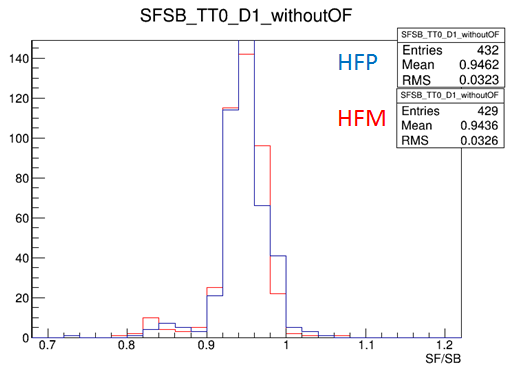
\includegraphics[width=.45\textwidth]{figures/ch_hfcalibration/SFSB_D1_woOF.png}
        }~
        \subfigure[]
        {
            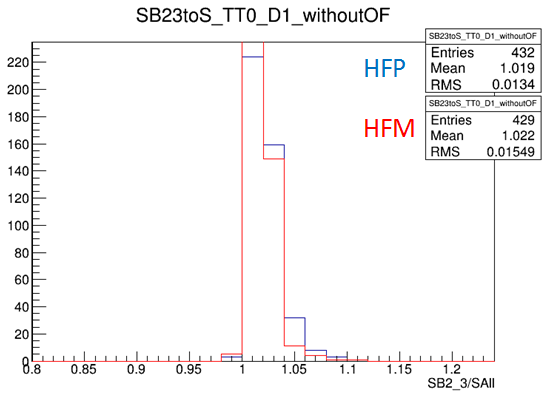
\includegraphics[width=.45\textwidth]{figures/ch_hfcalibration/SB23toS_D1_woOF.png}
        }
        \caption
        {(a) Ratio of the charge extracted from the "Front" region to the charge
         computed in the region "Back". Comparing Depth 1 or EM
         (b) Ratio of the charge computed within "2/3Back" region to the "Signal"
         region. Comparing Depth 1 or EM
         For both plots the compared quantity was the actual charge
         $Q$ADC/25\unit{ns}, excluding the overflow. Region are
         defined in the Table~\ref{tab:TubeRegions}}
        \label{fig:HF_LongUni}
    \end{center}
\end{figure}

\subsection{X-Checking}
An additional systematic uncertainty is included for the
methodology described in this note for measuring the absorber response to the source energy. Independent analyses were performed on the same data, and the results were compared and agree within an order of 1\%, as it can be deduced from figure~\ref{fig:Crosscheck}
\begin{figure}[!h]
    \begin{center}
        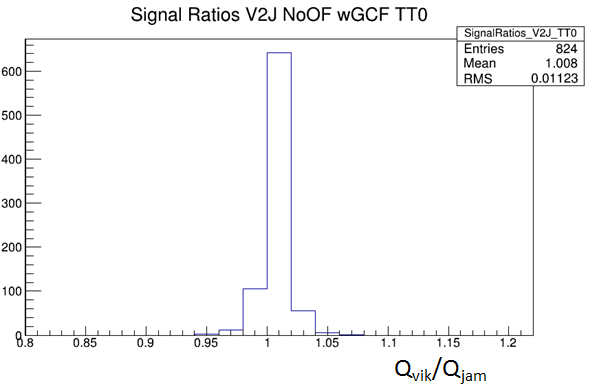
\includegraphics[width=.5\textwidth]{figures/ch_hfcalibration/Crosscheck.png}
        \caption{Cross-checking the results for HFM. On average the results agree
        within 1\%.}
        \label{fig:Crosscheck}
    \end{center}
\end{figure}
\section{Conclusions}
In this note we presented the results of the HF calorimeter sourcing calibration
procedure after new PMTs were installed on HF. Sourcing data was collected prior
to installing the new PMTs in HF- in order to obtain the average source energy
deposition and extrapolate over both HF calorimeters. Calibration coefficients
(HF Gains) were computed by averaging the background-subtracted signal yield
over the majority of the absorber depth (beyond 30cm of each end of the source
tube) for a given tower of each wedge and uploaded to the CondDB (Conditions
DataBase) for further use. Systematic uncertainties have been calculated and
estimated to be under 10\%, which agrees with the expected precision for our
calibration procedure.


% % Chapter Two - Apparatus
% \chapter{Apparatus} \label{chapter:Tables_and_Figures}

% This chapter describes the experimental apparatus and tools used to perform the analyses in this thesis.  For a fantastically detailed treatment of the LHC machine, see \cite{lhcMachine}.  See \cite{accelerators} for a thorough description of the physics and design of accelerators.

% \section{Introduction}
% 	The experimental apparatus described herein are located at CERN, on the outskirts of Geneva, Switzerland and across the borders of France and Switzerland.  CERN was first established in 1954, recently celebrating its 60th anniversary.  CERN has a diverse research program, all in support of studying the fundamental aspects of the universe, with an emphasis on providing state-of-the-art accelerator technology to its facilities and the world.  CERN has many secondary sites outside its main campus, the largest of which is the Prevessin site where the University of Iowa CMS group conducts its fixed target research activities.  See Figure \ref{fig:CERNMAP}    for a map of the CERN site.

% 	CERN is responsible for many technological achievements, including most famously the development of the World-Wide-Web by Tim Berners-Lee\cite{TBL}.  Many of the most important discoveries in particle physics have occurred at CERN, including the discovery of neutral currents\cite{currents}, the W and Z bosons\cite{WBoson}\cite{ZBoson}, the first creation of anti-hydrogen, the discovery of CP violation, and of course the observation of the Higgs Boson.

% 	The areas of most concern for this thesis include the LHC accelerator complex and the CMS experiment.

% 	\begin{figure}
% 		\begin{centering}
% 			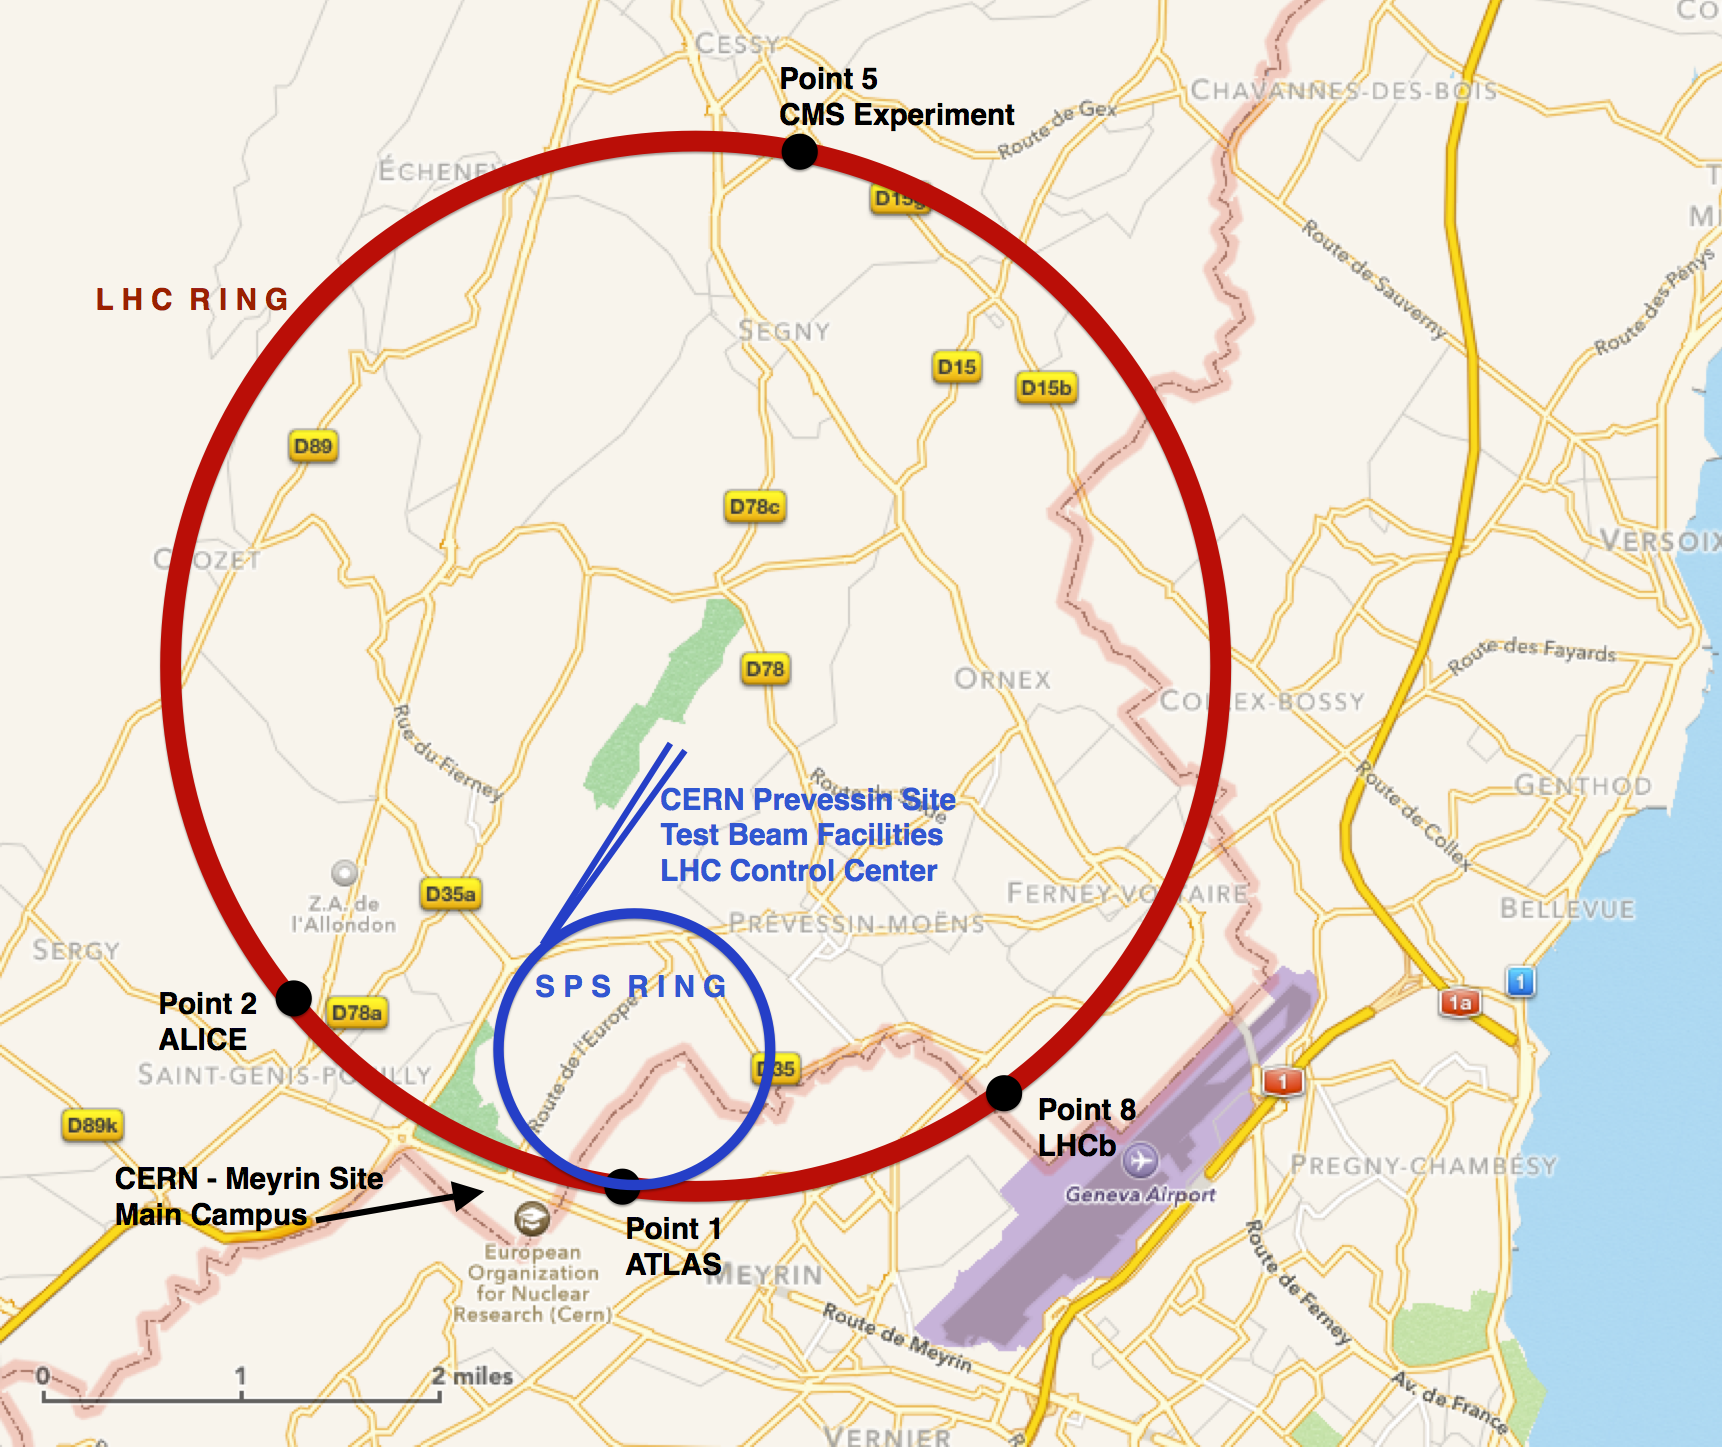
\includegraphics[scale=0.5]{figures/CERNMAP.png}
% 		\par\end{centering}
% 		\caption[Map of the CERN site]{\label{fig:CERNMAP}Map of the CERN site.  \textit{Map image courtesy of Apple Maps, Apple, Inc.}}
% 	\end{figure}


% \section{The Large Hadron Collider}
% In order to study the extremely short lived particles allowed by the universe, physicists need to recreate the exotic and controlled environments necessary to produce them.  The Large Hadron Collider at CERN was designed to collide protons at a center-of-mass energy of 14 tera-electronvolts (TeV).  Four separate collision halls were built to house four separate experiments: two general purpose detectors, ATLAS and CMS, and 2 specialty detectors, the b-quark-studying LHCb and the Pb-Pb collision-studying ALICE.  Dedicated \textit{heavy ion} runs are allocated during scheduled beam time, during which the protons in the beam pipe are evacuated and replaced with lead ions in order to study quark-gluon plasmas.

% 	\subsection{Principles of Design}
% 		The LHC's central feature is its accelerator system composed of a closed ring of 1232 superconducting dipole magnets supercooled to 1.9 Kelvin, evacuated to \(10^{-10}\) Torr, and positioned around the ring to sub-centimeter precision, totaling 27 km.  Figure \ref{fig:dipolexsec} shows a cross section of the main accelerator component, the LHC dipole magnet.  Figure \ref{fig:dipoleField} shows the incredible precision required of the B-field in order to steer the protons.  Table \ref{table:LHCtraits} lists the design characteristics of the LHC.

% 		Figure \ref{fig:acceleratorComplex} schematizes the CERN accelerator complex, including the dates that each accelerator came online.  The research accelerators of the past become the booster accelerators of the future.

% 		%%%%%%%%%%%%%%%%%%%%% LHC Dipole Magnet XSec %%%%%%%%%%%%%%%%%%%%%%%%%%%%%
% 		\begin{figure}
% 		\begin{centering}
% 			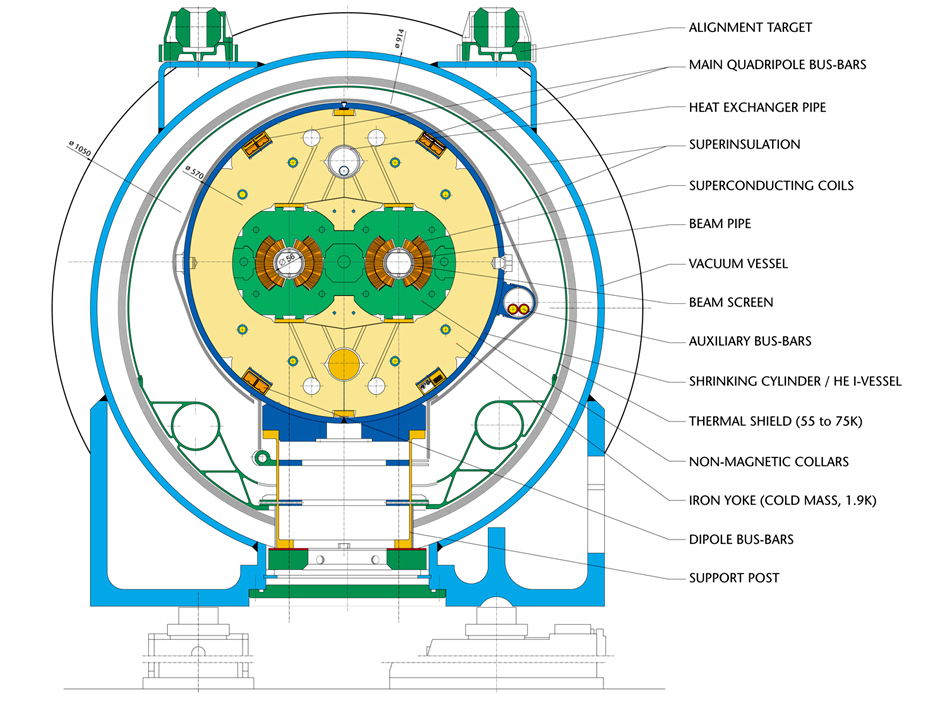
\includegraphics[scale=0.47]{figures/CH_2_a_The_LHC/dipolexsec.jpg}
% 		\par\end{centering}
% 		\caption[LHC Dipole Magnet Cross Section.]{\label{fig:dipolexsec}LHC Dipole Magnet Cross Section.  [CERN]}
% 		\end{figure}
% 		%%%%%%%%%%%%%%%%%%%%%%%%%%%%%%%%%%%%%%%%%%%%%%%%%%%%%%%%%%%%%%%

% 		%%%%%%%%%%%%%%%%%%%%% LHC Dipole Magnet Field %%%%%%%%%%%%%%%%%%%%%%%%%%%%%
% 		\begin{figure}
% 		\begin{centering}
% 			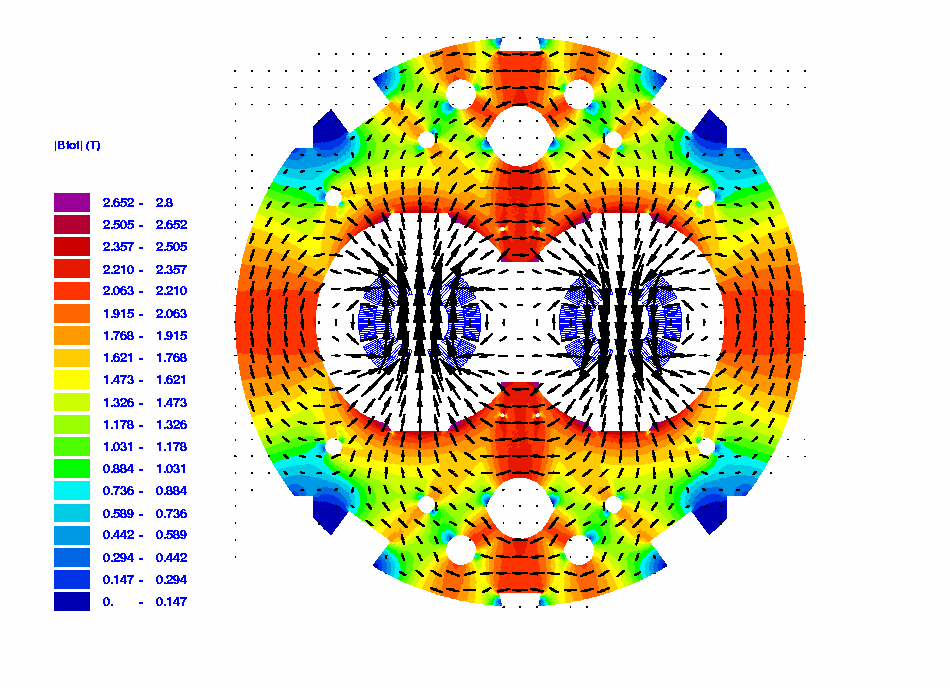
\includegraphics[scale=0.47]{figures/CH_2_a_The_LHC/LHC-Dipole-Magnetic-Field.png}
% 		\par\end{centering}
% 		\caption[LHC Dipole Magnet B-Field.]{\label{fig:dipoleField}LHC Dipole Magnet B-Field. [CERN]}
% 		\end{figure}
% 		%%%%%%%%%%%%%%%%%%%%%%%%%%%%%%%%%%%%%%%%%%%%%%%%%%%%%%%%%%%%%%%

% 		%%%%%%%%%%%%%%%%%%%%% LHC Dipole Magnet XSec %%%%%%%%%%%%%%%%%%%%%%%%%%%%%
% 		\begin{figure}
% 		\begin{centering}
% 			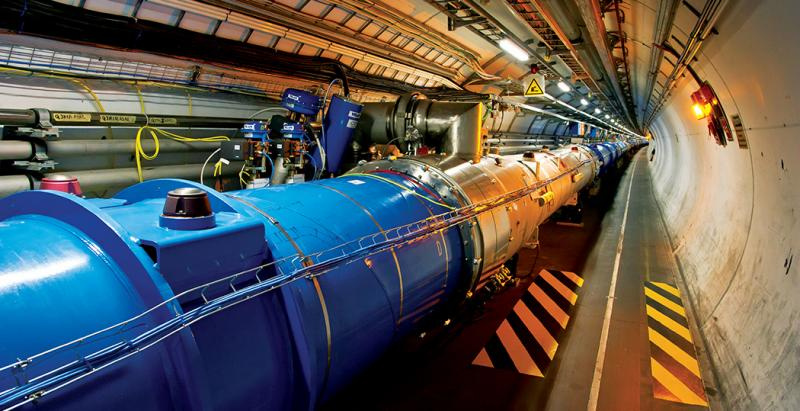
\includegraphics[scale=0.49]{figures/CH_2_a_The_LHC/lhc_long_1.jpg}
% 		\par\end{centering}
% 		\caption[Inside the LHC Accelerator Tunnel.]{\label{fig:lhcTunnel}Inside the LHC Accelerator Tunnel. [CERN]}
% 		\end{figure}
% 		%%%%%%%%%%%%%%%%%%%%%%%%%%%%%%%%%%%%%%%%%%%%%%%%%%%%%%%%%%%%%%%

% 		%%%%%%%%%%%%%%%%%%%%%%%%%%%%%%%%%% LHC Design Traits %%%%%%%%%%%%%%%%%%%%%%%%%%%%%%%
% 		\begin{table}
% 			\caption{Summary of the LHC design characteristics.}
% 			\label{table:LHCtraits}
% 			\begin{center}
% 				\begin{tabular*}{0.8\textwidth}{@{\extracolsep{\fill}}l  l}
% 					\hline
% 						\multicolumn{2}{c}{Machine Properties} 					\\
% 					\hline
% 					Circumference	 					& 27 km				\\
% 					Operating Temperature				& 1.9 K				\\
% 					Energy Usage						& 120 MW			\\
% 					Liquid Nitrogen Contained			& 10,800 Tons			\\
% 					Liquid Helium Contained				& 60 Tons				\\
% 					Tunnel Gradient					& 1.4\%				\\
% 					Beam Interlock Safety Signals			& Over 10,000			\\
% 					&\\
% 					\hline
% 						\multicolumn{2}{c}{Beam Properties}					\\
% 					\hline
% 					Collision Energy 					& 7 + 7 TeV			\\
% 					\(\gamma\) Factor 					& 7461				\\
% 					Luminosity						& \(10^{34}cm^{-2}s^{-1}\)	\\
% 					Injection Energy 					& 450 GeV			\\
% 					Beam Crossing Points  				& 4					\\
% 					Number of Bunches					& 2800				\\
% 					Number of Protons Per Bunch			& \(1.5\times 10^{11}\)	\\
% 					Time Spacing Per Bunch				& 25 ns				\\
% 					Beam Crossing Rate				& 40 MHz				\\
% 					Beam Current						& 2 ${\times}$ 0.58 A	\\
% 					Stored Energy						& 2 ${\times}$ 334 MJ	\\
% 					Bunch Width at Intersection			& 16.7 \(\mu m^2\)		\\
% 					Bunch Length at Intersection			& 11.24 cm			\\
% 					Amount of Steel for Magnet Yokes		& 55,000 Tons			\\
% 					Beam Velocity Magnitude				& 0.999999991 c		\\
% 					&\\
% 					\hline
% 						\multicolumn{2}{c}{Magnet Properties}					\\
% 					\hline
% 					Dipole Magnetic Field Strength 		& 8.4 T				\\
% 					Number of Main Dipole Magnets  		& 1232				\\
% 					Number of Quadrupole Magnets  		& 858				\\
% 					Number of Correcting Magnets			& 6208				\\
% 					Total Number of Magnets				& \~9300				\\
% 					Energy Stored Per Magnet			& 7 MJ				\\
% 					\hline
% 				\end{tabular*}
% 			\end{center}
% 		\end{table}
% 		%%%%%%%%%%%%%%%%%%%%%%%%%%%%%%%%%%%%%%%%%%%%%%%%%%%%%%%%%%%%%%%%%%%%%%%%%%%%%

% 		%%%%%%%%%%%%%%%%%%%%% LHC Accelerator Complex %%%%%%%%%%%%%%%%%%%%%%%%%%%%%
% 		\begin{figure}
% 		\begin{centering}
% 			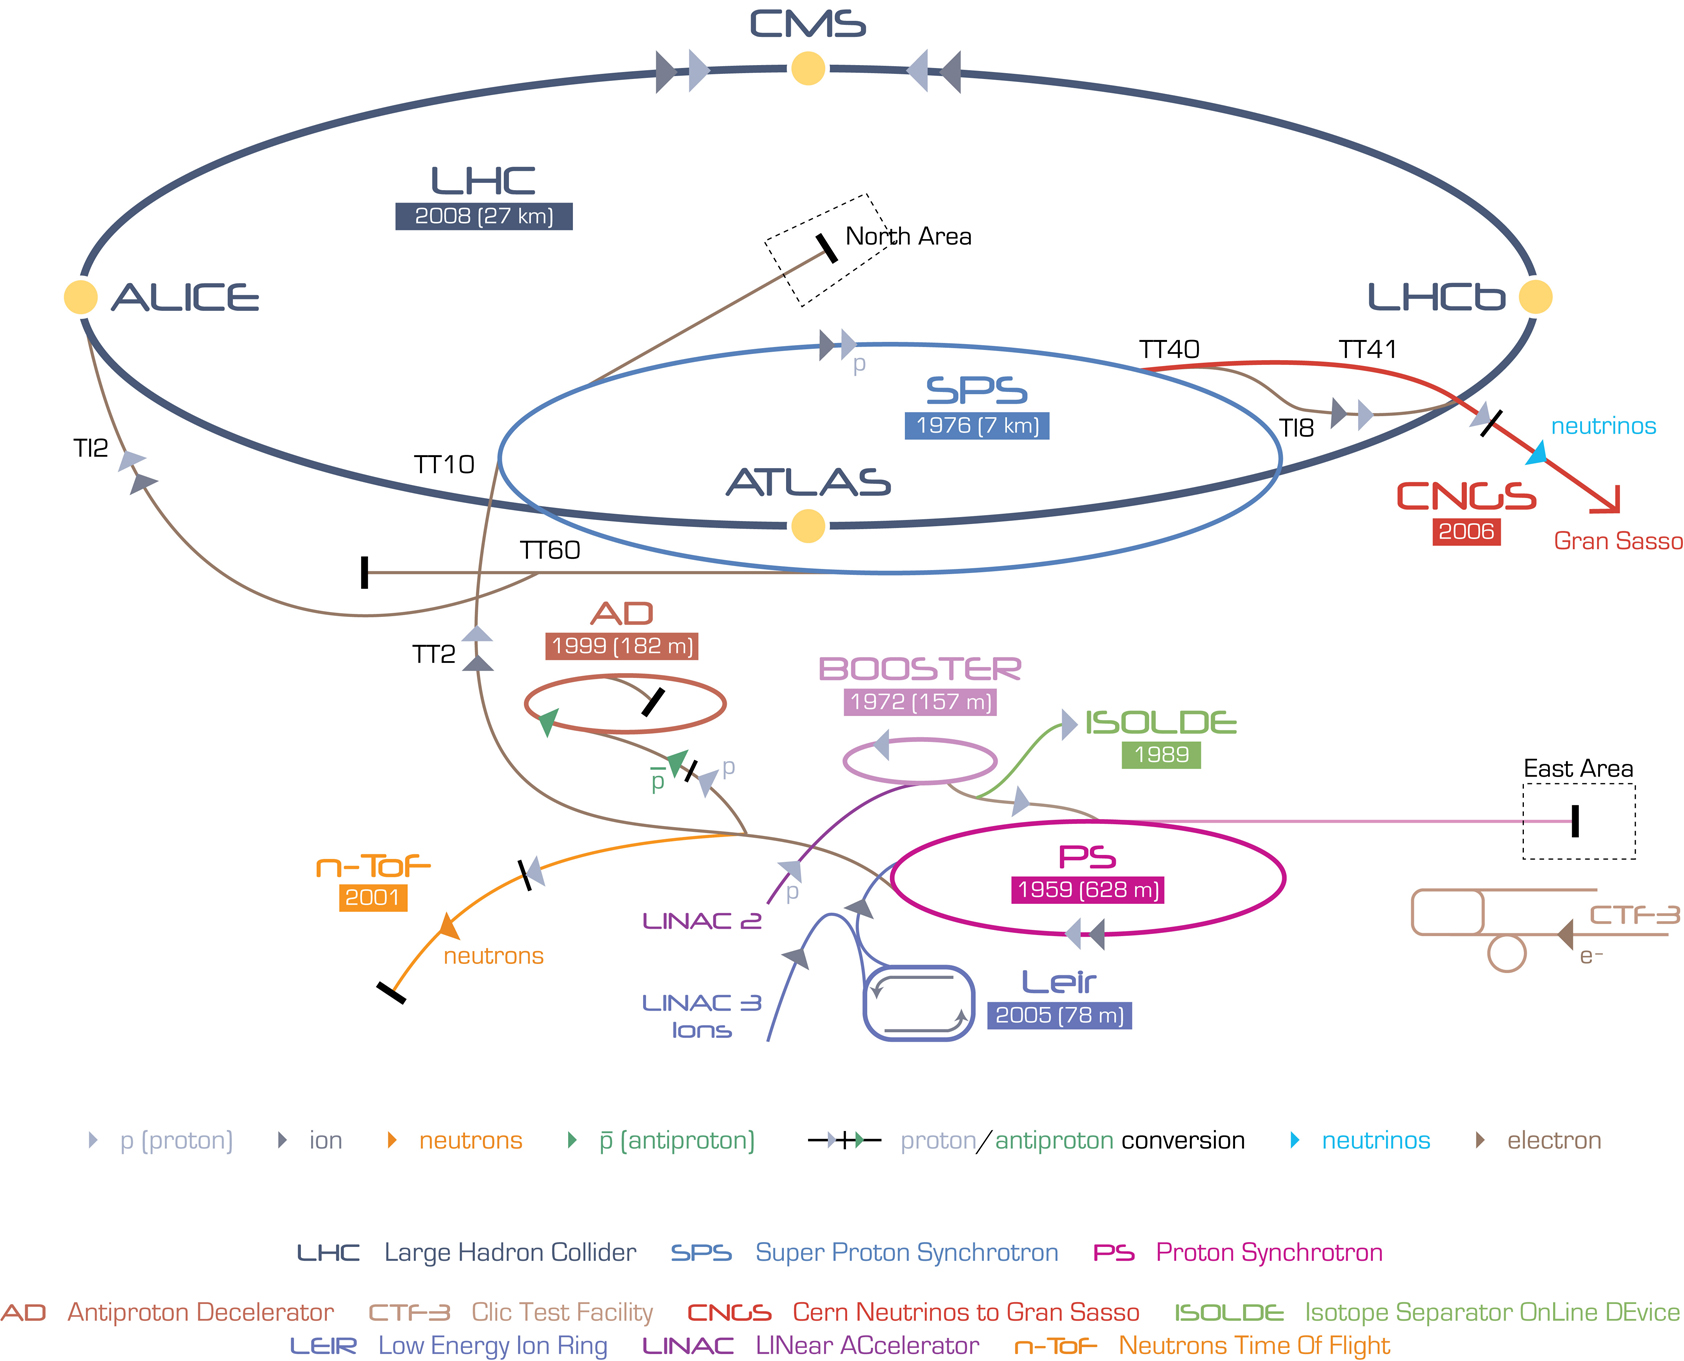
\includegraphics[scale=0.43]{figures/CH_2_a_The_LHC/Cern-Accelerator-Complex.jpg}
% 		\par\end{centering}
% 		\caption[The CERN Accelerator Complex.]{\label{fig:acceleratorComplex}The CERN Accelerator Complex. [CERN]}
% 		\end{figure}
% 		%%%%%%%%%%%%%%%%%%%%%%%%%%%%%%%%%%%%%%%%%%%%%%%%%%%%%%%%%%%%%%%


% 	\subsection{Proton Injection}
% 		Before any collisions can happen, a complex process of getting the protons to the interaction point must occur.  This sophisticated process begins with a tank of hydrogen gas, and not just any hydrogen gas, but hydrogen gas so pure the impurities are measured in parts per billion.  A 100 kV duoplasmatron collects the hydrogen gas and feeds it to a cathode chamber to strip off the electrons, yielding $\approx$ 70\% protons.   Magnetic fields compress and inject the protons at roughly 4,000 km/s (0.01$c$) into the LINAC2; see Figure \ref{fig:acceleratorComplex}.

% 		The protons then leave the LINAC2 with an energy of 50 MeV (0.31$c$) and enter the Proton Synchrotron Booster (PSB).  The PSB accelerates the protons to 1.4 GeV (0.92$c$)\footnote{At this energy, a proton is about 2.5 times more massive than at rest.} and injects the protons into the Proton Synchrotron (PS)\footnote{The PS was CERN's first accelerator, brought online in 1959.}.  The PS accelerates the protons to 25 GeV (0.9993$c$)\footnote{A proton is now almost 27 times more massive than it is at rest.}.

% 		The PS then hands the protons off to the Super Proton Synchrotron (SPS)\footnote{First turned on in 1976, this machine was responsible for the discovery of the W and Z bosons.} which accelerates the protons to 450 GeV (0.999998$c$)\footnote{A proton is now almost 500 times more massive than it is at rest.  Witness to the speed limit of the universe.}.

% 		After the SPS, the protons are injected into the LHC, which during the 2011 run, brought the protons to 3.5 TeV, 4 TeV during the 2012 run, and will bring them to the full design energy of 7 TeV (0.999999991$c$) during the 2015 run.


% 	\subsection{Beam Control}
% 		Controlling the LHC beam is a precise and involved task, with literally thousands of inputs that need to be tuned.  I invite the reader to consult \textit{LHC Beam Stability and Feedback Control} \cite{beamControl} for the methods and techniques beam scientists use to provide clean proton beams to the experiments.

% 		The LHC accelerator machine uses a system of alternating dipole and quadrupole magnets to accelerate and focus the proton beam.

% 		Figure \ref{fig:rfPhase} shows a longitudinal phase diagram for an accelerating RF system.  Particles are accelerated in bunches located in the blue region of Figure \ref{fig:rfPhase}, representing stability in phase space.


% 		%%%%%%%%%%%%%%%%%%%%%%%% RF  %%%%%%%%%%%%%%%%%%%%%%%%%%%%%%%%
% 		\begin{figure}
% 		\begin{centering}
% 			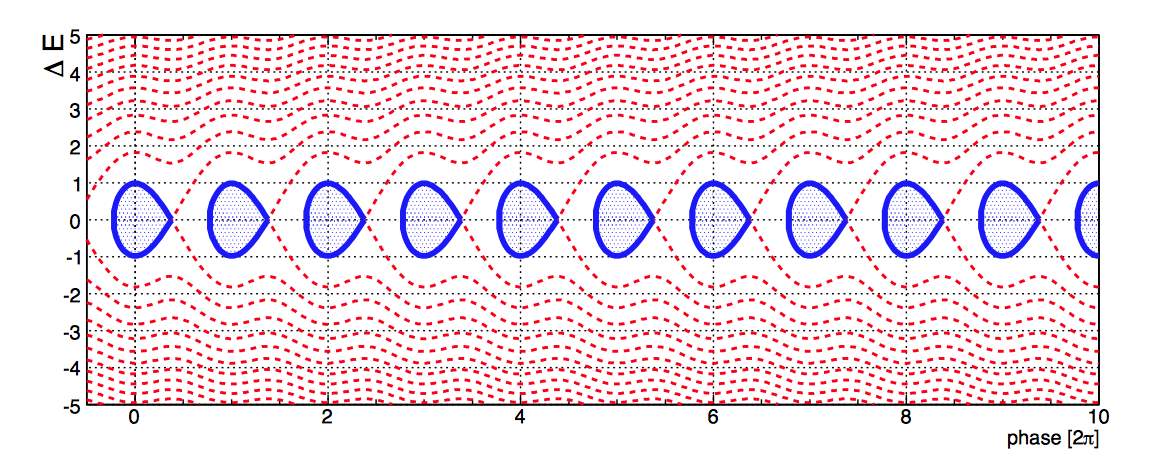
\includegraphics[scale=0.37]{figures/CH_2_a_The_LHC/RF_Phase.png}
% 		\par\end{centering}
% 		\caption[Longitudinal phase diagram for an accelerating RF system]{\label{fig:rfPhase}Longitudinal phase diagram for an accelerating RF system. [CERN]}
% 		\end{figure}
% 		%%%%%%%%%%%%%%%%%%%%%%%%%%%%%%%%%%%%%%%%%%%%%%%%%%%%%%%%%%%%%%%


% 		Some of the more bizarre concerns LHC beam physicists have to consider are thermal heating of the beam-pipe support girders, and distortion of the earth's crust due to lunar and solar gravitational forces.  The lunar perturbation affect has a periodicity of \(\approx\)25 hours.  The solar perturbation period is 24 hours with an effect \(\approx\)45\% that of the moon.  The secondary terrestrial tides result in a local shifting of the ground by \(\Delta a\)/\(a\) on the order of \(10^{-8}\) as shown in Figure \ref{fig:lunarSolar}.  The largest impact on the LHC occurs during \textit{spring tides}, when the sun and moon are on the same side of the Earth.  This results in a shift of the proton energy which causes the protons to move on a dispersion orbit on the order of 150\(\mu\)m.  This and other perturbations are compensated with beam stabilization techniques that include machine operator control tools like RF tuning, as well as automatic orbit feedback systems using beam position monitors and dipole corrector magnets.


% 		%%%%%%%%%%%%%%%%%%%%%%%% Lunar Solar  %%%%%%%%%%%%%%%%%%%%%%%%%%%%%%%%
% 		\begin{figure}
% 		\begin{centering}
% 			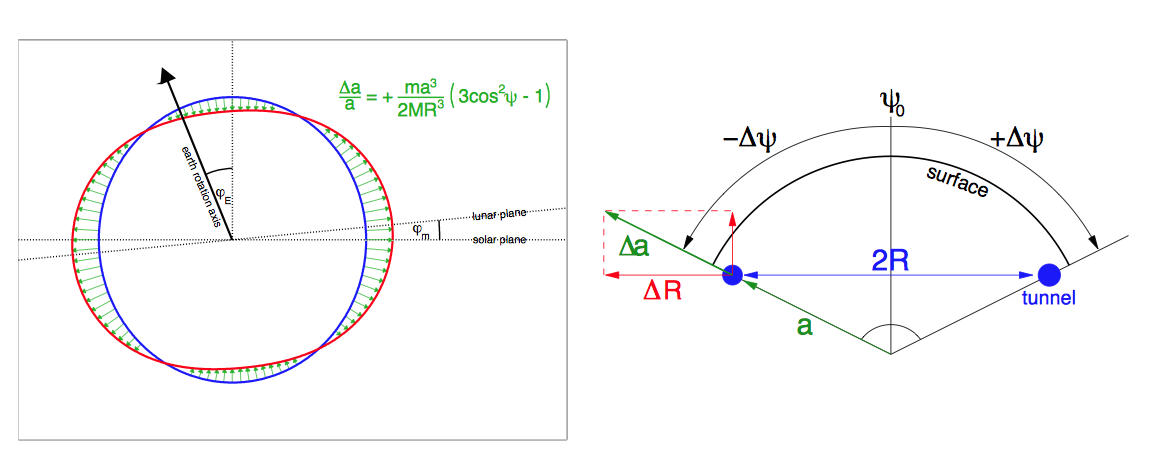
\includegraphics[scale=0.4]{figures/CH_2_a_The_LHC/LunarSolar.png}
% 		\par\end{centering}
% 		\caption[Tidal deformation of the Earth's surface (left) and resulting LHC tunnel deformation (right).]{\label{fig:lunarSolar}Tidal deformation of the Earth's surface (left) and resulting LHC tunnel deformation (right).  This diagram is not to scale. [CERN]}
% 		\end{figure}
% 		%%%%%%%%%%%%%%%%%%%%%%%%%%%%%%%%%%%%%%%%%%%%%%%%%%%%%%%%%%%%%%%


% 		%%%%%%%%%%%%%%%%%%%%%%%% CMS Detector  %%%%%%%%%%%%%%%%%%%%%%%%%%%%%%%%
% 		\begin{figure}[H]
% 		\begin{centering}
% 			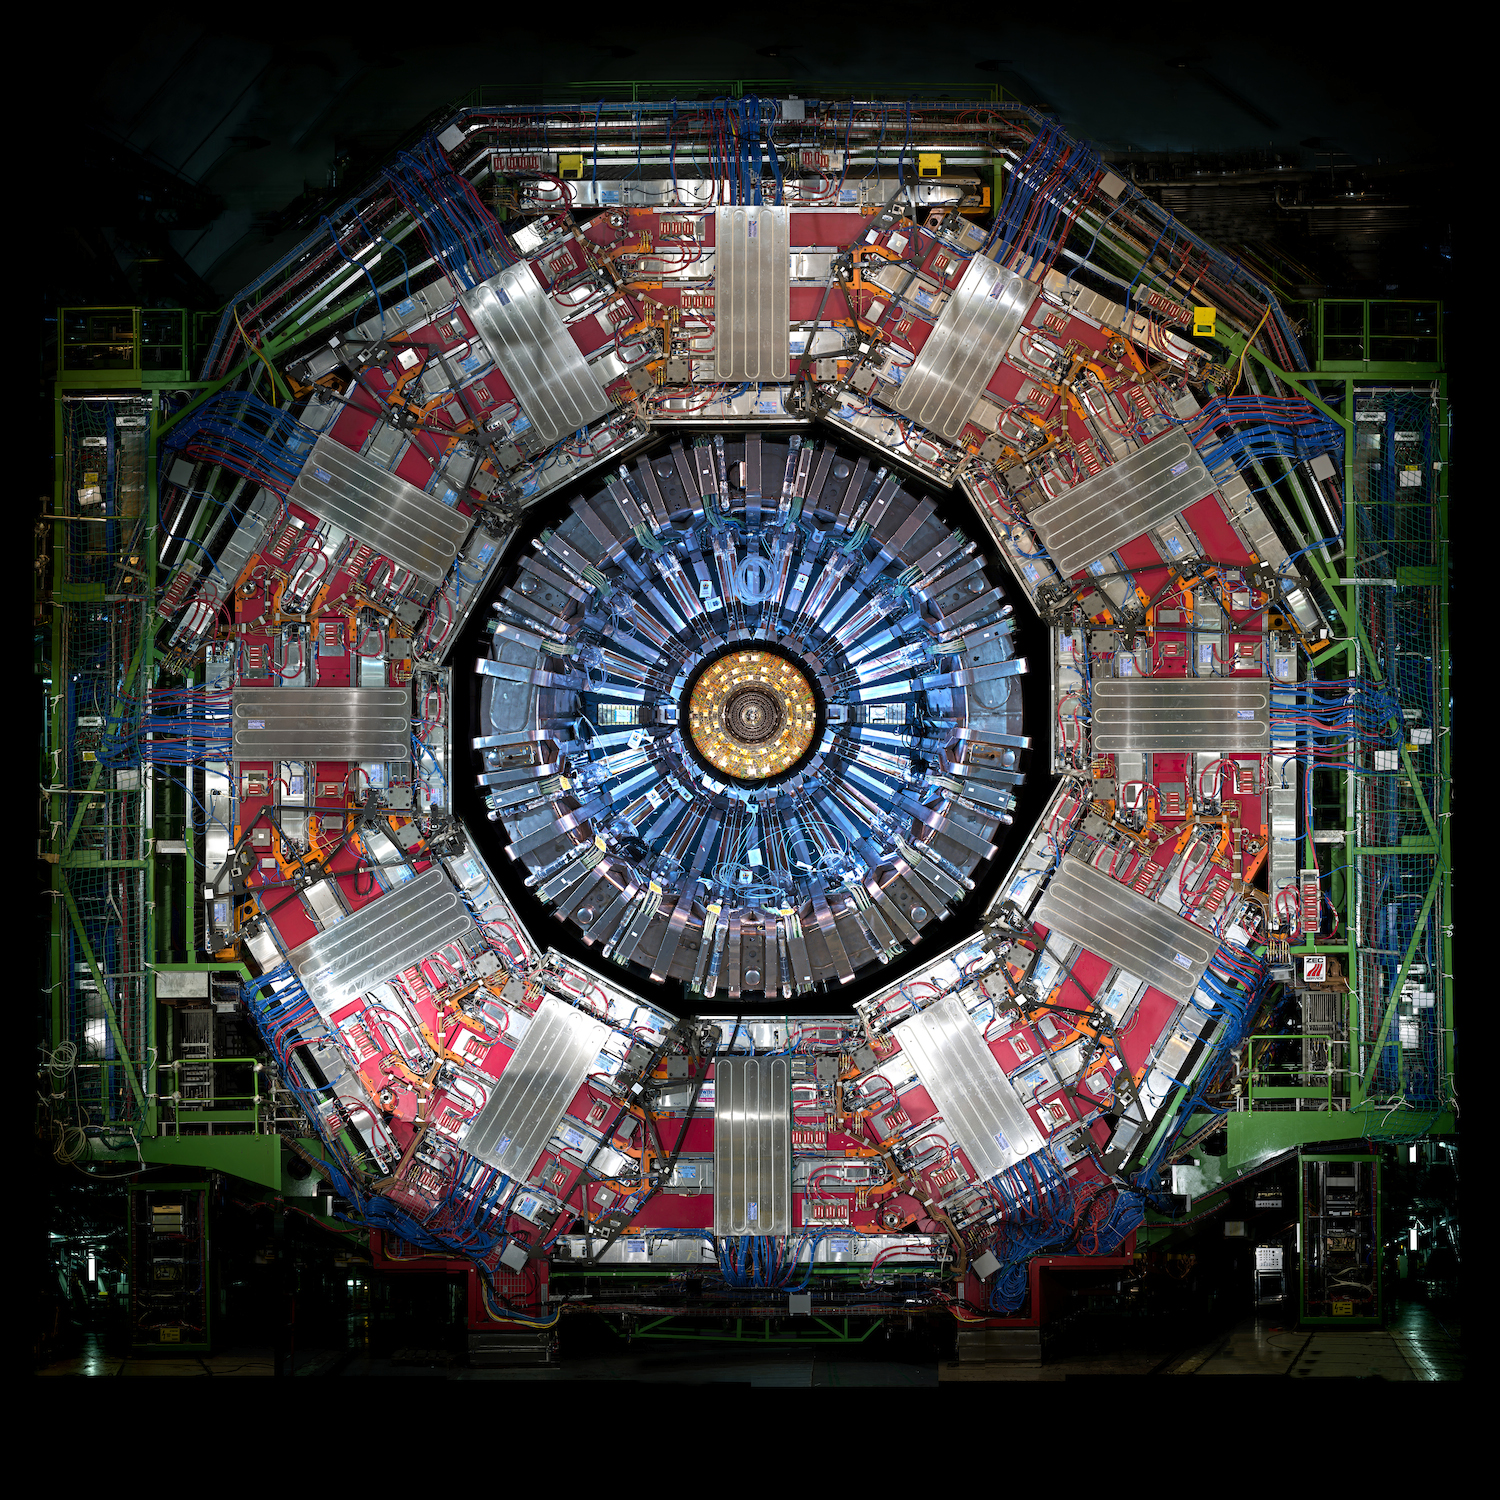
\includegraphics[scale=0.28]{figures/CH_2_b_CMS/CMS.jpg}
% 		\par\end{centering}
% 		\caption[The CMS detector in the experimental cavern.]{\label{fig:CMS}The CMS detector in the experimental cavern. [CERN]}
% 		\end{figure}
% 		%%%%%%%%%%%%%%%%%%%%%%%%%%%%%%%%%%%%%%%%%%%%%%%%%%%%%%%%%%%%%%%

% \section{The Compact Muon Solenoid Detector}
% The CMS Detector is the main experimental apparatus responsible for collecting the data used for the analysis chapter of this thesis, and whose detector elements are the subject of the hardware chapter.  The \textit{Technical Design Report} (TDR)\cite{TDR} of the CMS detector is an excellent resource for those interested in a more thorough treatment of the detector elements.

% 	\subsection{Principles of Design}
% 		The CMS detector is one of two \textit{general purpose} detectors, along with ATLAS, on the LHC.  CMS is a \(4\pi\) detector, meaning in principle it is able to reconstruct collisions with full r/rho/phi coverage around the interaction point.  CMS is an initialism for Compact Muon Solenoid:
% 		\bigskip
% 		\begin{description}
% 			\item[Compact] for its density of detector elements.
% 			\item[Muon] due to the large role, both in the physical design and the physics goals, that muons and the muon detectors play.
% 			\item[Solenoid] for the massive 4 Tesla magnet system at the heart of the detector.
% 		\end{description}

% 		\bigskip

% 		Figure \ref{fig:CMS} is an image of the CMS detector, without its end caps in place\footnote{A main design goal of the CMS collaboration was to ensure, despite its compactedness, easy access to detector elements for upgrade and maintenance.  Each slice of CMS can be moved independently by forcing pressurized air through its feet, giving it just enough lift to be pushed around.}.  It is the view of the detector a proton would see, looking right down the beam line.  Figure \ref{fig:CMSLabelled} is an isometric cutaway view of CMS, with each of its subdetectors labelled.

% 		A common coordinate system is defined in CMS for locating elements in the detector for use within software and for engineering purposes.

% 		\begin{itemize}
% 			\item The \textit{z-axis} is defined as the axis along the beam-line, with $z=0$ at the interaction point.  The positive z-direction is from side R56 towards R54, or directionally West towards the Jura mountains.
% 			\item The \textit{x-axis} points towards the center of the LHC.
% 			\item The \textit{y-axis} is defined as straight up from the interaction point.
% 			\item The angle $\phi$, referred to as the \textit{azimuthal angle}, is measured from the $x$-axis in the $x-y$ plane, where $\phi=0$ points towards the center of the LHC ring with radial component $r$.
% 			\item The polar angle $\theta$ is defined in the $rz$ plane.
% 			\item The \textit{pseudorapidity} is defined as $\eta = -$ln (tan$(\theta/2)$), and is useful due to the Lorentz invariance of the opening angle between particles.
% 		\end{itemize}

% 		The sub-detectors of CMS are the tracker, electromagnetic calorimeter (ECAL), hadronic calorimeter (HCAL), and muon system.  As a particle travels from the interaction point through the detector, each detector subsystem is responsible for a part of its reconstruction.  See Figure \ref{fig:particleFlow} for a diagram of the particle flow in CMS and how different particles respond to the different subdetectors.

% 		%%%%%%%%%%%%%%%%%%%%%%%% CMS Detector Labeled %%%%%%%%%%%%%%%%%%%%%%%%%%%
% 		\begin{figure}
% 		\begin{centering}
% 			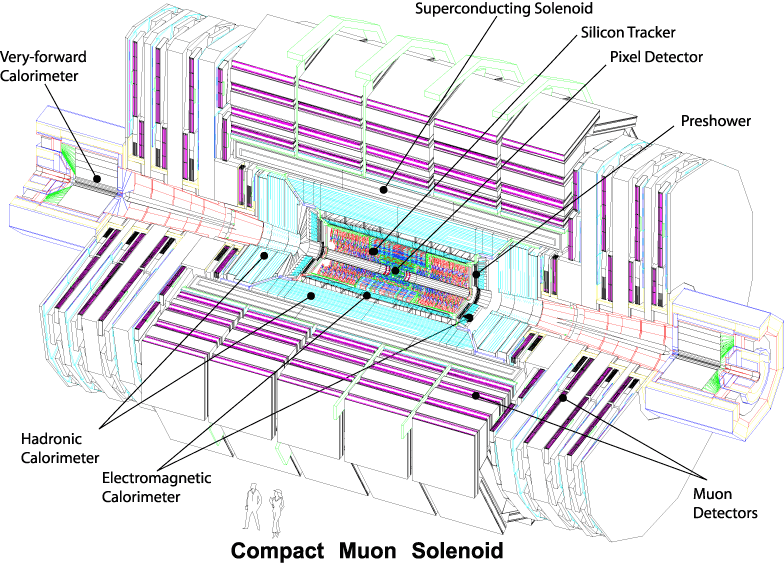
\includegraphics[scale=0.5]{figures/CH_2_b_CMS/cms_labelled.png}
% 		\par\end{centering}
% 		\caption[Cutaway isometric view of the CMS detector]{\label{fig:CMSLabelled}Cutaway isometric view of the CMS detector. [CERN]}
% 		\end{figure}
% 		%%%%%%%%%%%%%%%%%%%%%%%%%%%%%%%%%%%%%%%%%%%%%%%%%%%%%%%%%%%%%%%


% 		%%%%%%%%%%%%%%%%%%%%%%%%  Particle Flow  %%%%%%%%%%%%%%%%%%%%%%%%%%%
% 		\begin{figure}
% 		\begin{centering}
% 			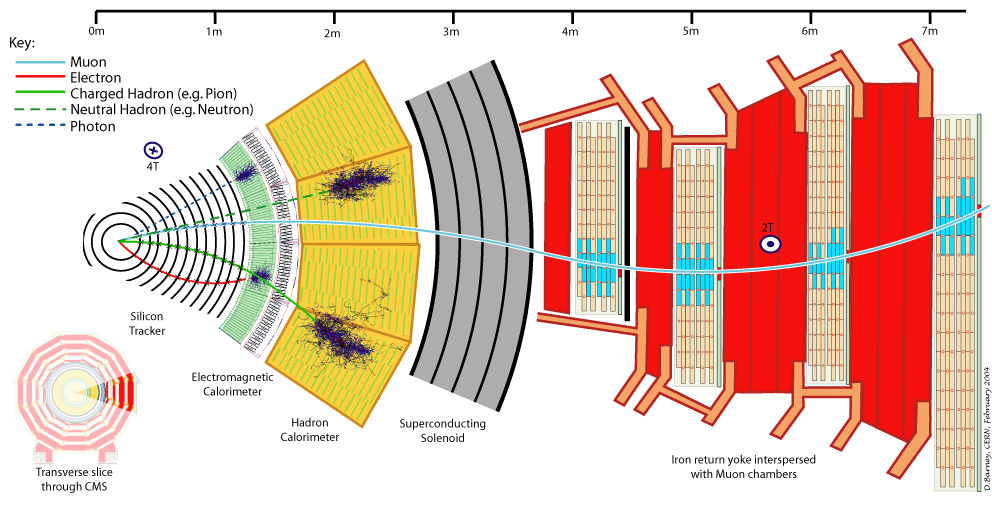
\includegraphics[scale=0.4]{figures/CH_2_b_CMS/CMS_Slice.png}
% 		\par\end{centering}
% 		\caption[Particle flow in the CMS Detector.]{\label{fig:particleFlow}Particle flow in the CMS Detector. [CERN]}
% 		\end{figure}
% 		%%%%%%%%%%%%%%%%%%%%%%%%%%%%%%%%%%%%%%%%%%%%%%%%%%%%%%%%%%%%%%%

% 		The tracker system is designed to record precision tracks of the particles to help identify individual particle momentum by precisely fitting their trajectories.  The ECAL and HCAL systems are designed to measure the energies of the particles.  The muon system has the very difficult job of reconstructing muons.  The detector software has to stitch the signals from each of these detectors together to create the reconstructed particle objects used for analysis.


% 		%%%%%%%%%%%%%%%%%%%%%%%% CMS Tracker System %%%%%%%%%%%%%%%%%%%%%%%%%%%%
% 		\begin{figure}[H]
% 		\begin{centering}
% 			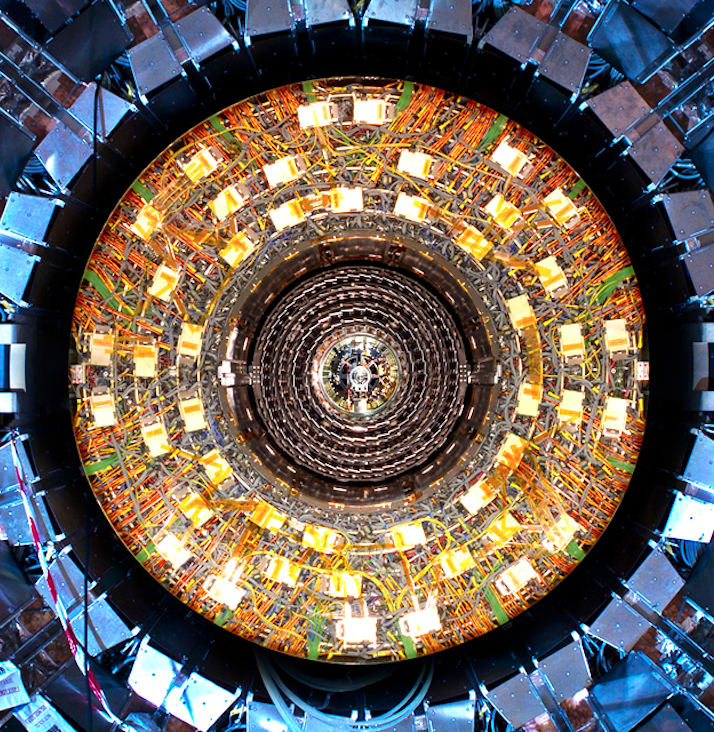
\includegraphics[scale=0.4]{figures/CH_2_b_CMS/CMS_Tracker.png}
% 		\par\end{centering}
% 		\caption[The CMS Tracking System viewed along the beam line.]{\label{fig:CMSTracker}The CMS Tracking System viewed along the beam line. [CERN]}
% 		\end{figure}
% 		%%%%%%%%%%%%%%%%%%%%%%%%%%%%%%%%%%%%%%%%%%%%%%%%%%%%%%%%%%%%%%%


% 	\subsection{Inner Tracker}
% 		The main goal of the tracking system in CMS is to record the initial trajectories of the particles prior to reaching the calorimeter systems allowing the precise measurement of the particles' paths and momentums.
% 		The inner tracker system has a total active area of over 200m$^2$, and is composed of two main subsystems:  the pixel detector (within 0.2m of the beam pipe) and the silicon strip detector (between 0.2-1.2m from the beam pipe), as seen in Figure \ref{fig:CMSTracker}.
% 		The pixel detector is composed of 1440 pixel modules totaling 66 million individual pixels.  The silicon strip detector contains 15,148 modules containing 9.3 million readout channels.

% 		Precise reconstruction of collision vertices is a major tool to limit pileup contamination.  Pileup is a term used to describe the amount of extemporaneous particles in a detector beyond those of interest in the main event.  Pileup is due to the nature of proton-proton collisions and the high luminosity of the collision environment, causing several interactions in each event.  The higher the beam luminosity, the greater the pileup.  The tracking system is used to precisely reconstruct interaction vertices, limiting the effects of pileup.

% 		Because of its close proximity to the beam line and the high flux of particles to which it is exposed, the tracker system will be the first CMS sub-detector to be replaced due to radiation damage.  Despite the peril of its proximity, its closeness to the interaction point is the tracker system's greatest asset.

% 		%%%%%%%%%%%%%%%%%%%%%%%% CMS Tracker System2 %%%%%%%%%%%%%%%%%%%%%%%%%%%%
% 		\begin{figure}
% 		\begin{centering}
% 			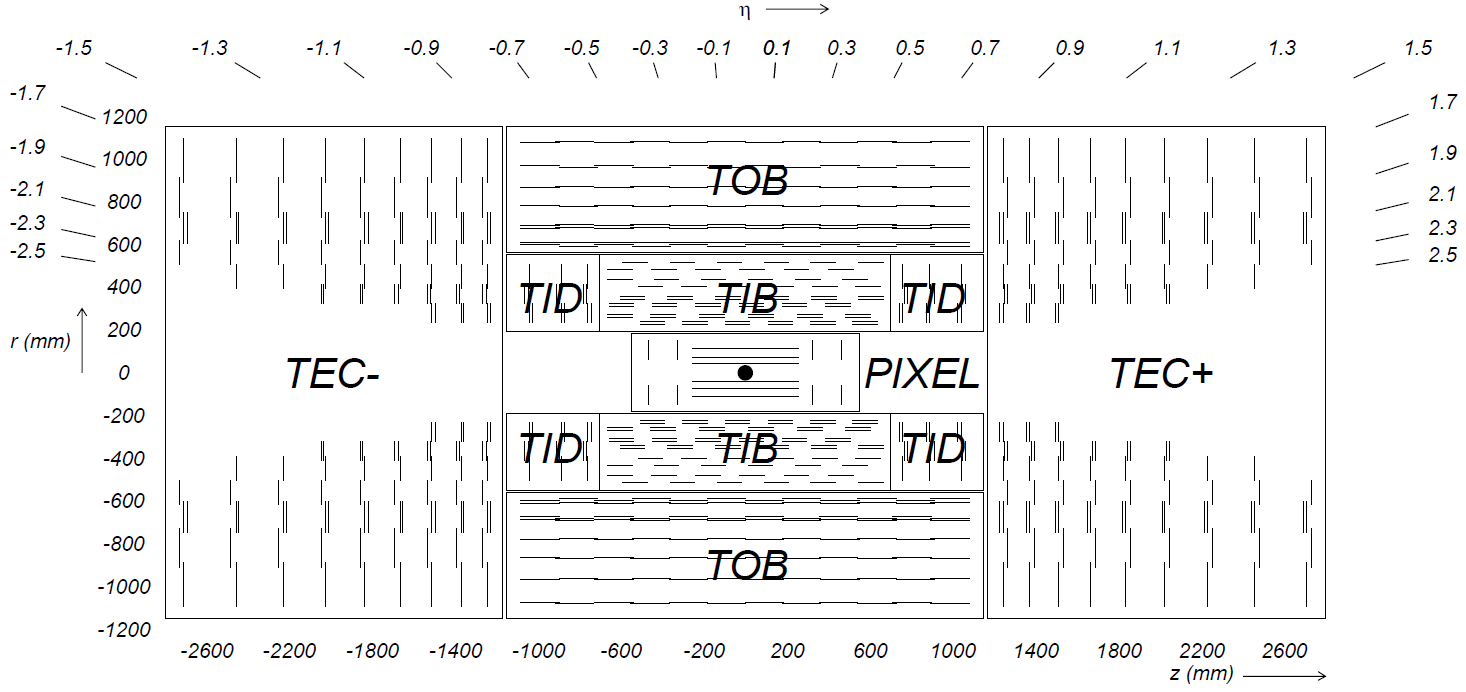
\includegraphics[scale=0.3]{figures/CH_2_b_CMS/CMS_Tracker2.png}
% 		\par\end{centering}
% 		\caption[The CMS Tracking system schematic.]{\label{fig:CMSTracker2}The CMS Tracking system shematic.  Each line represents a layer of active detector elements.  The submodules listed represent the inner barrel (TIB), outer barrel (TOB), inner disc (TID), and endcap regions (TEC). [CERN]}
% 		\end{figure}
% 		%%%%%%%%%%%%%%%%%%%%%%%%%%%%%%%%%%%%%%%%%%%%%%%%%%%%%%%%%%%%%%%

% 		%%%%%%%%%%%%%%%%%%%%%%%% CMS Strip Tracker %%%%%%%%%%%%%%%%%%%%%%%%%%%%
% 		\begin{figure}
% 		\begin{centering}
% 			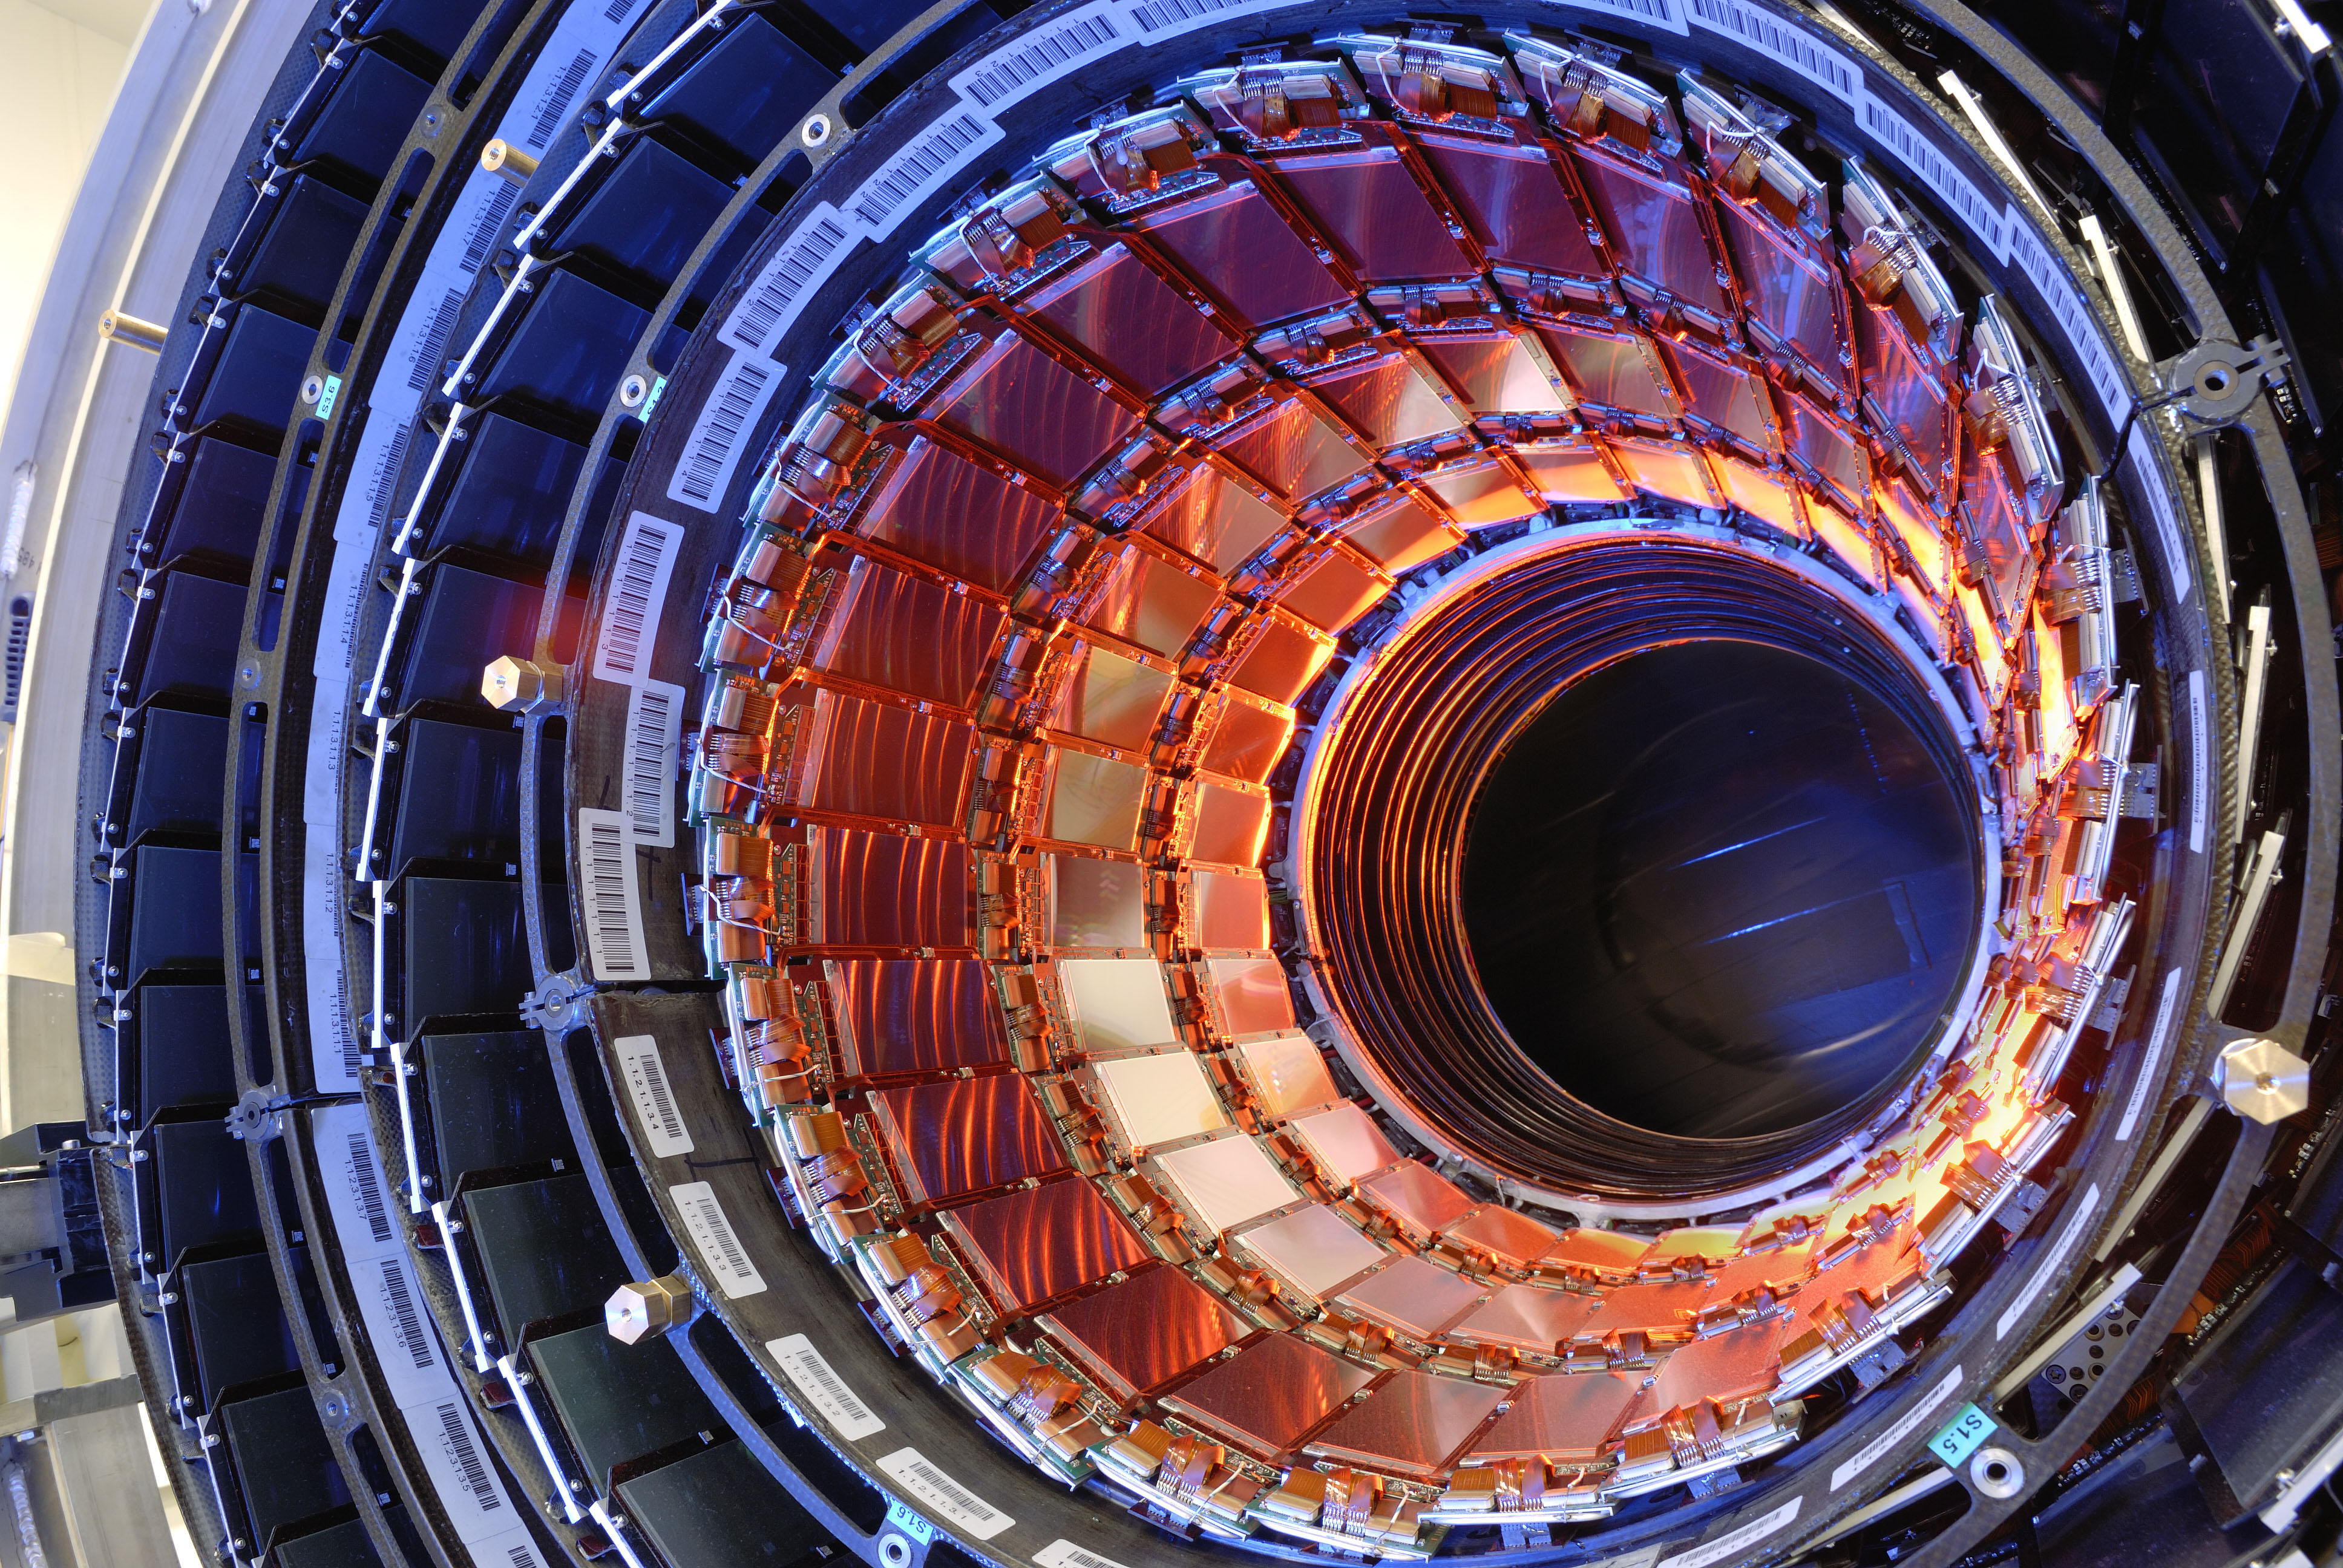
\includegraphics[scale=0.45]{figures/CH_2_b_CMS/CMS_StripTracker.jpg}
% 		\par\end{centering}
% 		\caption[The silicon strip \textit{inner barrel} of the CMS tracking system.]{\label{fig:CMSStripTracker}The silicon strip \textit{inner barrel} of the CMS tracking system. [CERN]}
% 		\end{figure}
% 		%%%%%%%%%%%%%%%%%%%%%%%%%%%%%%%%%%%%%%%%%%%%%%%%%%%%%%%%%%%%%%%

% 		%Ecal picture Francesca Cavallari


% 		%%%%%%%%%%%%%%%%%%%%%%%% CMS ECAL Installation %%%%%%%%%%%%%%%%%%%%%%%%%%%
% 		\begin{figure}[H]
% 		\begin{centering}
% 			\includegraphics[scale=0.5]{figures/CH_2_b_CMS/CMS_ECAL_Install.jpg}
% 		\par\end{centering}
% 		\caption[Italian physicist Francesca Cavallari beneath the ECAL Barrel.]{\label{fig:CMSEcalInstall}Italian physicist Francesca Cavallari beneath the ECAL Barrel. [CERN]}
% 		\end{figure}
% 		%%%%%%%%%%%%%%%%%%%%%%%%%%%%%%%%%%%%%%%%%%%%%%%%%%%%%%%%%%%%%%%


% 	\subsection{Electromagnetic Calorimeter}
% 		The ECAL Barrel (EB) system's central detector element is a 2.2 $\times$ 2.2 $\times$ 23 cm$^3$  lead tungstate (PbWO$_4$) crystal, read out by avalanche photo diodes (APDs) with an active area of 5 $\times$ 5 mm$^2$.  The response of an APD to an electron changes by 3.8\%/\degree C, requiring a water cooling system in ECAL to maintain a nominal temperature of 18\degree C, and be monitored to a precision of $\pm$0.05\degree C.

% 		The ECAL Endcap (EE) system also uses lead tungstate crystals with a slightly different geometry, 2.86 $\times$ 2.86 $\times$ 22 cm$^3$, read out with vacuum phototriodes (VPT).

% 		Figure \ref{fig:CMSECALcutaway} is a schematic view of the ECAL system, showing the `D' shaped endcaps (each half referred to as a `\textit{Dee}'), and the central barrel.  The cutaway also shows off the PbWO$_4$ crystal arrangement visible as the finely segmented regions in the upper cutaway of the barrel, and horizontally oriented along the edge of the dee end-cap, on the left of the schematic.  Notice the change in gradient of the crystals as they get further from the interaction point (the center of the 3D object).


% 		%%%%%%%%%%%%%%%%%%%%%%%% CMS ECAL %%%%%%%%%%%%%%%%%%%%%%%%%%%%%%%%%%%%%%%%%%
% 		\begin{figure}[H]
% 		\begin{centering}
% 			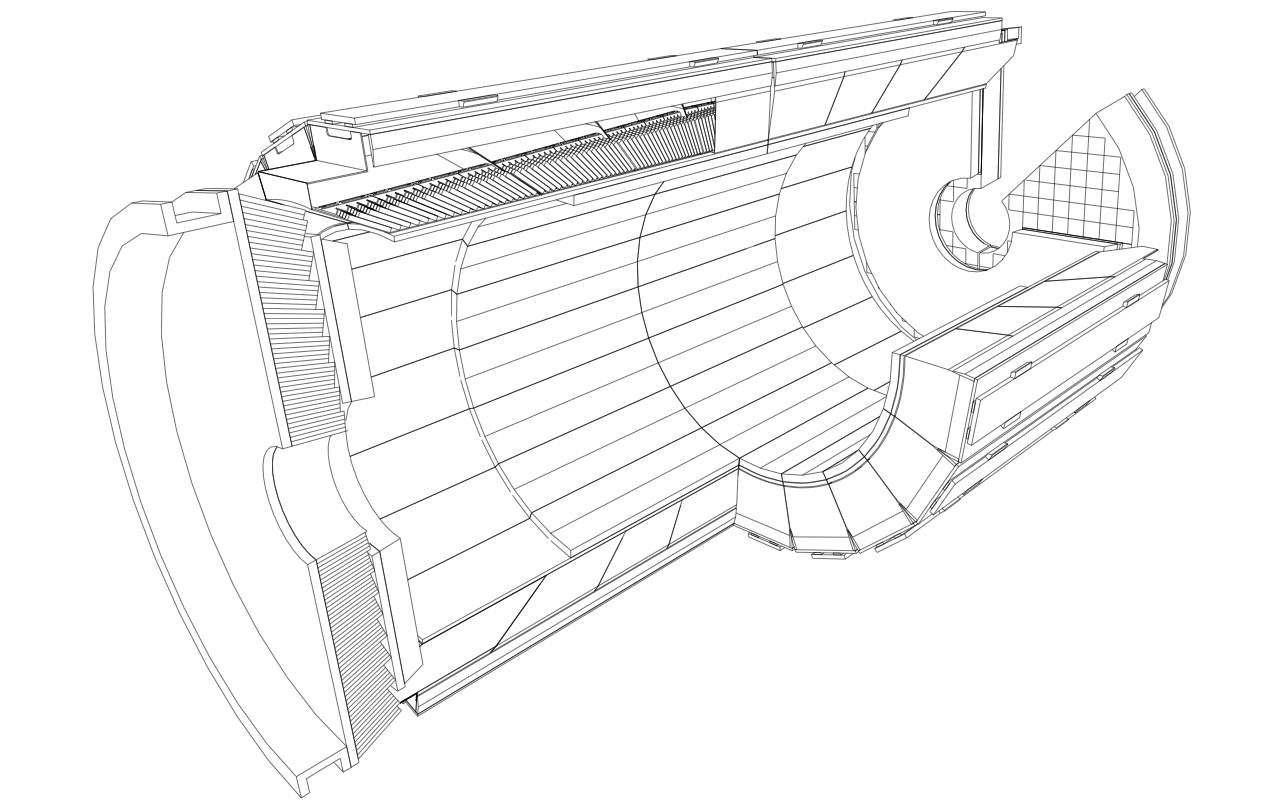
\includegraphics[scale=0.35]{figures/CH_2_b_CMS/CMS_ECAL_cutaway.png}
% 		\par\end{centering}
% 		\caption[ECAL cutaway showing endcap (EE) and barrel (EB) subdetectors.]{\label{fig:CMSECALcutaway}ECAL cutaway showing endcap (EE) and barrel (EB) subdetectors. [CERN]}
% 		\end{figure}
% 		%%%%%%%%%%%%%%%%%%%%%%%%%%%%%%%%%%%%%%%%%%%%%%%%%%%%%%%%%%%%%%%%%%%%%%%%


% 		The ECAL system contains 75,848 PbWO$_4$ crystals in order to have high energy resolution and reconstruction ability.  A charged particle passing into the crystal will cause a shower which in turn will cause the crystal to scintillate, depositing its light into the photodetector at the back of the crystal.  See Figure \ref{fig:CMSECALShower} for a simulation of a 24 GeV electron entering a crystal.


% 		%%%%%%%%%%%%%%%%%%%%%%%% CMS ECAL Shower %%%%%%%%%%%%%%%%%%%%%%%%%%%%%%%%%%%%%
% 		\begin{figure}
% 		\begin{centering}
% 			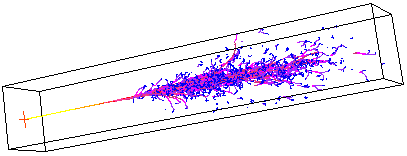
\includegraphics[scale=0.8]{figures/CH_2_b_CMS/CMS_ECAL_Shower.png}
% 		\par\end{centering}
% 		\caption[ECAL PbWO$_4$ crystal shower simulation of a 24 GeV $e^-$.]{\label{fig:CMSECALShower}ECAL PbWO$_4$ crystal shower simulation of a 24 GeV $e^-$. [CERN]}
% 		\end{figure}
% 		%%%%%%%%%%%%%%%%%%%%%%%%%%%%%%%%%%%%%%%%%%%%%%%%%%%%%%%%%%%%%%%%%%%%%%%%


% 	%%%%%%%%%%%%%%%%%%%%%%%% CMS HCAL Shells %%%%%%%%%%%%%%%%%%%%%%%%%%%%%%%%%%%%%%
% 	\begin{figure}[H]
% 	\begin{centering}
% 		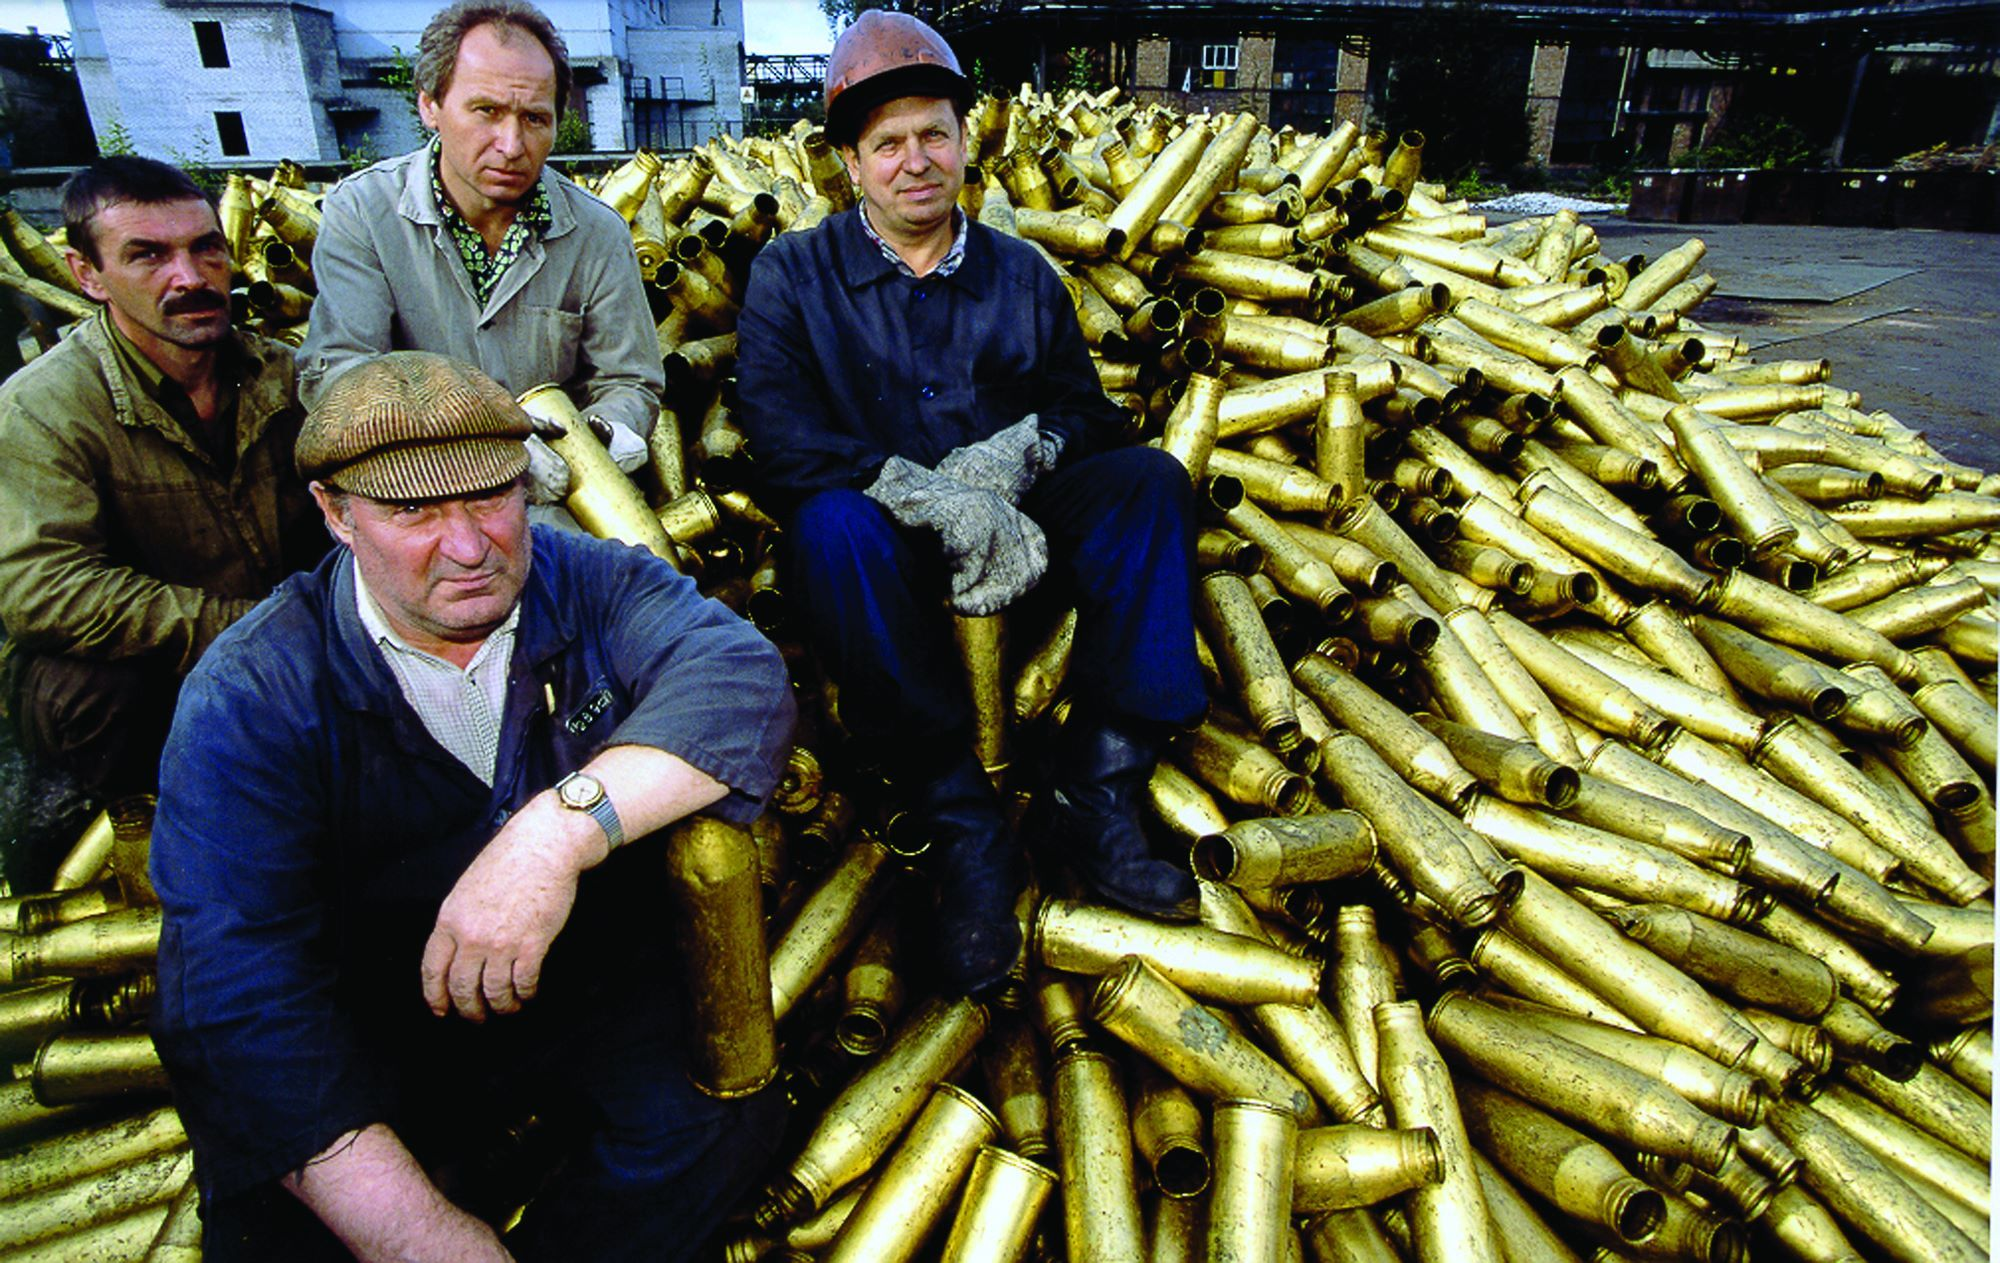
\includegraphics[scale=0.2]{figures/CH_2_b_CMS/CMS_HCAL_shells.jpg}
% 	\par\end{centering}
% 	\caption[Russian Navy shells used to create the brass tiles of HCAL.]{\label{fig:CMSHCALShells}Russian Navy shells used to create the brass tiles of HCAL.  Over one million brass shell casements were melted down for use in the HCAL detector.  [CERN]}
% 	\end{figure}
% 	%%%%%%%%%%%%%%%%%%%%%%%%%%%%%%%%%%%%%%%%%%%%%%%%%%%%%%%%%%%%%%%%%%%%%%%%


% 	\subsection{Hadronic Calorimeter}
% 	The HCAL system is composed of three main subsystems\cite{HCAL}:
% 	\begin{description}
% 		\item[HB:] Hadronic Barrel $\eta < 1.3$
% 		\item[HO:] Hadronic Outer $\eta < 1.3$
% 		\item[HE:] Hadronic Endcap $1.3 > \eta < 3$
% 		\item[HF:] Hadronic Forward $3 > \eta < 5.2$
% 	\end{description}
% 	\bigskip

% 	Figure \ref{fig:CMSHCALShells} is an image of a Russian crew responsible for decommissioning over one million Russian Navy brass shell casements leftover from WWII.  The Russia and Dubna Member States (RDMS) collaboration was responsible for sourcing the material to be used in HCAL.  Military grade brass turned out to have exactly the right properties, so an agreement was struck between the Russian Navy and CMS to turn over the more than one million shells\footnote{This actually was not enough material to meet the 650 tons of brass required by HCAL.  The remaining material was donated by the US, totalling over \$1 million USD.}.

% 	HCAL is a sampling calorimeter composed of brass wedges embedded with scintillating tiles.  Wavelength shifting fibers are embedded in the scintillator tiles to carry the light generated in the tile by the particles to the hybrid photodiodes for signal readout.  The plastic scintillator tiles will not withstand the radiation environment;  replacement technology is being actively researched.


% 	%%%%%%%%%%%%%%%%%%%%%%%% CMS Muon System %%%%%%%%%%%%%%%%%%%%%%%%%%%%%%%%%%%%%%
% 	\begin{figure}[H]
% 	\begin{centering}
% 		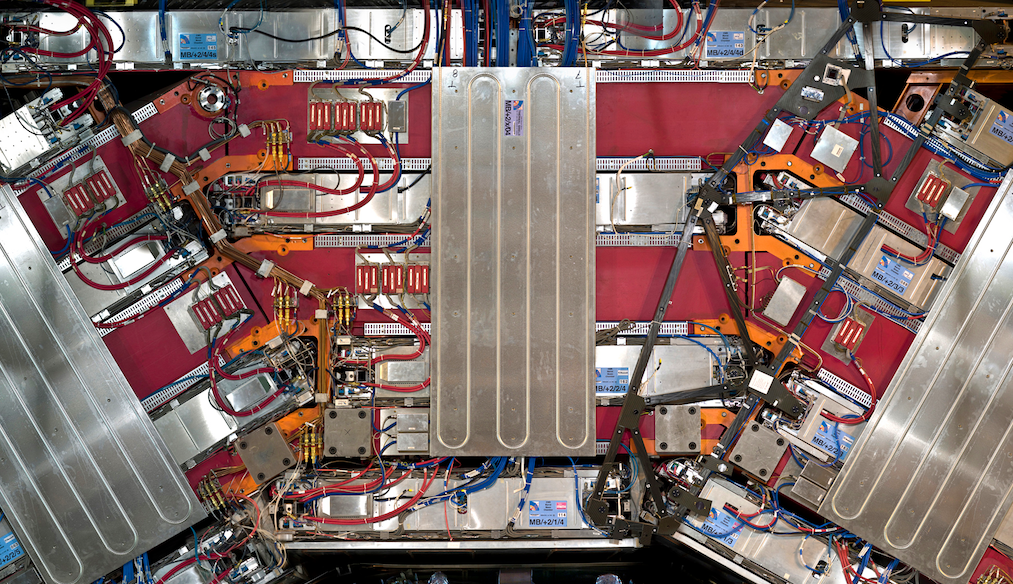
\includegraphics[scale=0.4]{figures/CH_2_b_CMS/CMS_MuonSystem.png}
% 	\par\end{centering}
% 	\caption[A segment of the CMS muon system.]{\label{fig:CMSMuonSystem}A segment of the CMS muon system.  RPCs and DTs (silver) interspersed between the iron magnet return yokes (red). [CERN]}
% 	\end{figure}
% 	%%%%%%%%%%%%%%%%%%%%%%%%%%%%%%%%%%%%%%%%%%%%%%%%%%%%%%%%%%%%%%%%%%%%%%%%


% 	\subsection{Muon System}
% 		A central feature of the CMS detector is the muon detector system; see Figure \ref{fig:CMSMuonSystem}.  The muon system can be divided into three main sub-units:
% 		\begin{description}
% 			\item[RPC:] Resistive Plate Chambers
% 			\item[DT:]	Drift Tubes
% 			\item[CSC:] Cathodic Strip Chambers
% 		\end{description}
% 		\bigskip

% 		The RPCs and DTs are used in the barrel region of CMS, while the RPCs and CSCs are used in the end-cap region, see Figure \ref{fig:CMSMuonSchematic}.  DTs cannot be used in the end-cap region due to the non-homogeneity of the magnetic field; see Figure \ref{fig:CMSBField}.


% 		%%%%%%%%%%%%%%%%%%%%%%%% CMS Muon System Schematic%%%%%%%%%%%%%%%%%%%%%%%%%%%%%%%%%
% 		\begin{figure}
% 		\begin{centering}
% 			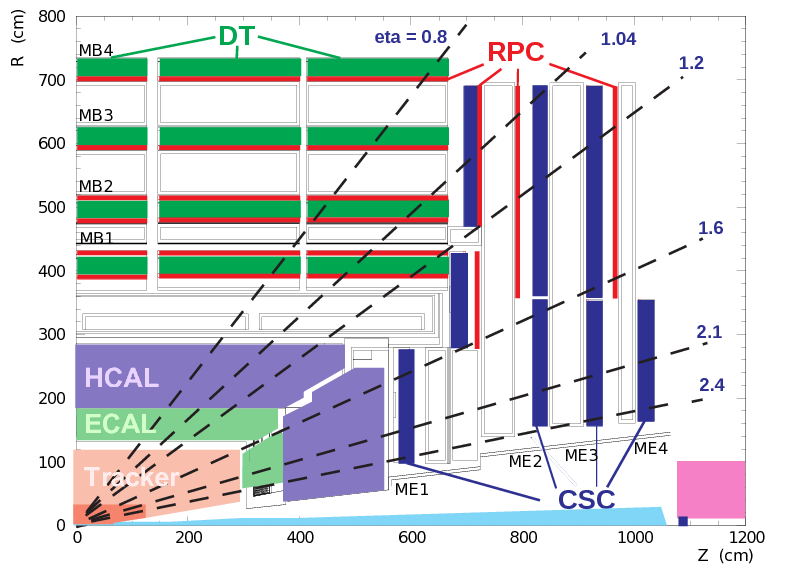
\includegraphics[scale=0.4]{figures/CH_2_b_CMS/CMS_Muon_schematic.png}
% 		\par\end{centering}
% 		\caption[Longitudinal quadrant view of the CMS muon system.]{\label{fig:CMSMuonSchematic}Longitudinal quadrant view of the CMS muon system. [CERN]}
% 		\end{figure}
% 		%%%%%%%%%%%%%%%%%%%%%%%%%%%%%%%%%%%%%%%%%%%%%%%%%%%%%%%%%%%%%%%%%%%%%%%%


% 		%%%%%%%%%%%%%%%%%%%%%%%% CMS Magnet System %%%%%%%%%%%%%%%%%%%%%%%%%%%%%%%%%%%%%
% 		\begin{figure}
% 		\begin{centering}
% 			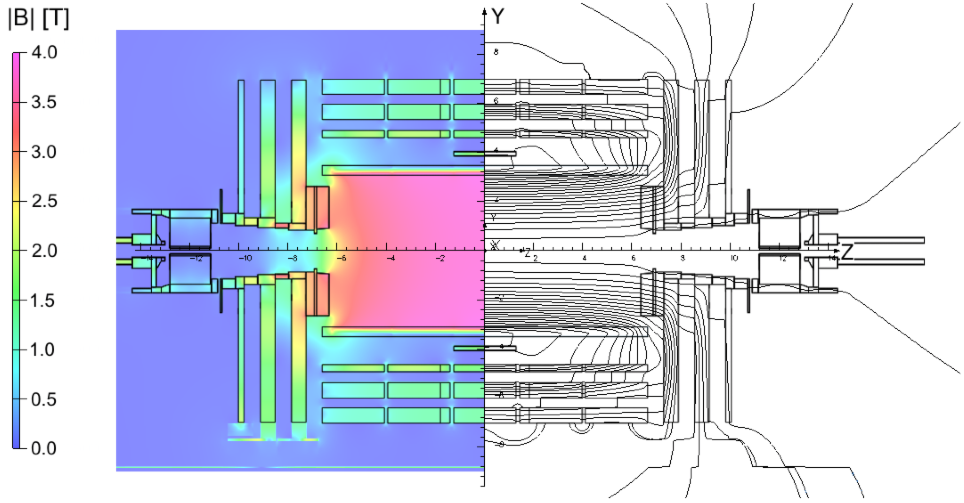
\includegraphics[scale=0.4]{figures/CH_2_b_CMS/CMS_Solenoid.png}
% 		\par\end{centering}
% 		\caption[Simulated strength (left) and field lines (right) of the B-field in CMS.]{\label{fig:CMSBField}Simulated strength (left) and field lines (right) of the B-field in CMS.}
% 		\end{figure}
% 		%%%%%%%%%%%%%%%%%%%%%%%%%%%%%%%%%%%%%%%%%%%%%%%%%%%%%%%%%%%%%%%%%%%%%%%%


% 	\subsection{Trigger}
% 		The target event rate for recorded data in CMS is 100Hz.  The LHC is designed to deliver more than 20 interactions every 25 ns.  The electronics operate at a frequency of $\sim 10^9$Hz and have about $\sim 10^8$ channels to be readout, creating raw data at a rate on the order of 100 TB every second.  The CMS trigger system has the daunting task of reducing this data rate to 100MB/s without discarding meaningful events.  This job is left to the Level 1 (L1) Trigger and the High Level Trigger (HLT).

% 		The HLT can only handle a data input rate of 100 kHz, requiring the L1 trigger to reduce the raw detector data rate by a factor of 10,000.  The L1 trigger processes an event every 3.2$\mu$s, requiring the detector to store a buffer of events totaling 128 bunch crossings.  The L1 trigger makes its decisions taking input from the calorimeter trigger, the muon trigger, the global trigger, and the TTC (timing, trigger, and control system).

% 		The HLT has roughly 1 second to make a final decision on an event passed by the L1 trigger, and can therefore incorporate the full calorimeter granularity and tracker system into the decision making process.  The goal here is to reduce the event rate further by a factor of 1,000.

% 	\subsection{CMS Software}\label{Section:CMSSW}
% 		This section describes the software tools used for the studies contained within this thesis.  The CMS Experiment has developed a coherent set of data simulation, processing, and analysis software known as CMS Software, or CMSSW.  CMSSW is a modular framework written almost entirely in C++ and Python.  CMSSW was developed entirely alongside the ROOT analysis framework.  ROOT is an object oriented analysis package utilizing objects to contain data.  This makes the task of handling CMS data much simpler and more powerful.

% 		The backbone of the CMSSW system is a class-based architecture known as The Event Data Model, or EDM.  Central to CMSSW is the idea of an \textit{Event} in CMS, in both the literal and virtual sense.  For example, a real muon reconstructed in CMS is referred to as a \textit{physics object} in both the muon software class and in the actual detector.

% 		Information in an event can only be manipulated independently by discrete \textit{modules}, where most often the modules need to be executed on the data in a particular order, as the necessary data formats may not yet exist in the event.  The various modules can be grouped into six separate categories, as follows:

% 		\begin{description}
% 			\item[Source:] The source modules most generally import RAW data from the detector in the form of a ROOT file in the ROOT data format, though it is modular enough to take in custom data formats.  In the case of MC generation, the source is used as a container to hold the generated events before being processed by other modules.

% 			\item[EDProducer:]  RAW data from CMS is generally not very useful to physicists doing analysis, so EDProducers are used to produce \textit{Event Data}.  Example packages would turn raw hits from the Tracker into a collection of reconstructed \textit{tracks}, which could be used by another EDProducer module to reconstruct an electron from the tracks.  In this case, the causal nature of the EDProducers is apparent.

% 			\item[EDFilter:] Often times a user will want to remove an event or kill a process that is not useful.  The EDFilter reads a single event and returns a boolean that is used by the framework to determine whether or not to continue the process.  An example is the process \textit{StopAfterNEvents}, which will kill the \textit{process path} after reaching the critical number of events set by the user.  Another, NTrackFilter, might kill the event if too many tracks are reconstructed.

% 			\item[EDAnalyzer:] Once the data has been processed and the preferred data formats obtained, a physicist will want to analyze the events without adding or removing information to the event.  An EDAnalyzer module is used to analyze events without altering them, and is typically used to create output histograms in the ROOT format, although any format can be used if programmed by the user.

% 			\item[EDLooper:] Occasionally a physicist will find themselves wanting to tune some parameters and re-processing the source multiple times.  The EDLooper is used for this.

% 			\item[OutputModule:] After all analysis is done, an OutputModule is used to write the data from an event to an external source.  Most commonly, \textit{PoolOutputModule} is used to write the output data to a ROOT file.
% 		\end{description}

% 		\bigskip
% 		All object classes and data formats are defined within a given CMSSW release, with versions ranging from CMSSW\_1\_1\_1 up to CMSSW\_7\_0\_0 and beyond, with custom releases for studying specific features or testing upgrades of CMS routinely developed and maintained.  CMSSW is housed in a git repository on GitHub\cite{github}.  The analysis in this thesis uses CMSSW\_5\_3\_8.

% 	\subsection{CMSSW and CMS Simulation}\label{section:fullsim}
% 		The entire CMS detector has been modeled in the software package GEANT4 and interfaced with CMSSW.  There are two main detector simulation and modeling packages:
% 		\begin{itemize}
% 			\item Full Simulation
% 			\item Fast Simulation
% 		\end{itemize}

% 		Full simulation is termed \textit{fullSim} and encodes every aspect of CMS into GEANT4, from cabling, detector materials, to detector component efficiencies and noise simulations.  This can make for extremely long simulation run-times.  As a particle is stepped through the detector, each property is simulated, from its interaction with the detector, to possible showering, and the resulting detector response.  A single event can take as much as 20 minutes to be modeled.  Considering that a minimum event set is generally required to be on the order of five thousand events, it can take more than 24 hours to generate a dataset of this size.

% 		Fast simulation is nicknamed \textit{fastSim} and is a parameterization of detector characteristics based on several runs of the more realistic fullSim, test beam results, and other studies.  The advantage is lower run times for simulations while maintaining real detector responses.  Instead of simulating the detector response with every step a particle takes, a parameterization is used that can range from a lookup table, to a functional, or an ntuple.


% \section{Particle Identification}
% 	The CMS Particle Object Groups (POG) are responsible for determining how the detector signals from the previously described detector elements should be reconstructed into real physics objects to be used by physicists in their analysis.  The following describes the processes involved with determining the particles in the final state of the search described in Chapter \ref{HMNSearch}.

% 	\subsection{Muon Reconstruction}
% 		There are three main methods to reconstruct muons.  The first uses the CMS tracker, referred to as \textit{tracker muons}.  The second uses the main muon subsystem consisting of the RPCs, DTs, and CSCs, referred to as \textit{standalone muons}.  The third and most complete method combines the information from the tracker system and the muon system.

% 		\begin{description}
% 		\item[Tracker Muons:]  Track seeds produced in the PIXEL detector are propagated to the rest of the detector volume by connecting the tracks to form a trajectory.

% 		\item[Standalone Muons:] Muon hits in the individual layers of RPCs and DTs or CSCs are stitched together to form trajectories.

% 		\item[Global Muons:]  A global fit is applied to the trajectory created between hits in the tracker system and the muon system.
% 		\end{description}

% 		The equations of motion for a charged particle (like the muon) through CMS is written as:
% 		\begin{equation}
% 			\frac{d^2\vec{r}}{ds^2} = \frac{q}{p}\frac{d\vec{r}}{ds}\times \vec{B}(\vec{r})
% 		\end{equation}

% 		Given that $\vec{B} = B\hat{z}$ in CMS and choosing $ds^2 = dx^2 + dy^2 + dz^2$, the equations of motion can be written as:
% 		\begin{equation}
% 			x(s) = x_0 + R_H[cos(\phi_0 + h\cdot s\cdot cos(\lambda / R_H) - cos(\phi_0))]
% 		\end{equation}
% 		\begin{equation}
% 			y(s) = y_0 + R_H[sin(\phi_0 + h\cdot s\cdot cos(\lambda/R_H) - sin(\phi_0))]
% 		\end{equation}
% 		\begin{equation}
% 			z(s) = z_0 + s\cdot sin(\lambda)
% 		\end{equation}
% 		\begin{equation}
% 			R_H = \frac{p\cdot cos(\lambda)}{qB}
% 		\end{equation}
% 		\begin{equation}
% 			\lambda = arcsin(\frac{dz}{ds})
% 		\end{equation}

% 		where $R_H$ is the helix radius, $\phi_0$ is the azimuthal angle with respect to the helix axis, and $\lambda$ is the slope angle.

% 		This general method is applied in each muon reconstruction algorithm, along with the Kalman filter extrapolation procedure \cite{kalman} which matches a set of hits in one layer to hits in a neighboring layer with algorithms that account for uncertainties (like position resolution) and multiple scattering.

% 		This analysis requires muons to both be \textit{global} muons and satisfy so-called \textit{particle-flow ID} requirements, explained in Section \ref{sec:particleFlow}.

% 	\subsection{Jet Reconstruction}\label{section:jets}
% 		Jets are complex objects that show up in the detector as large deposits of energy in the calorimeters, resulting from the hadronization of hard parton scattering, even including photons and electrons.  It is therefore important for the CMS software to do a good job in reconstructing and categorizing the jet objects in the CMS detector.

% 		There are several algorithms used to tag jets; this analysis uses the \textit{anti-$k_T$} algorithm.  Each algorithm uses a combination of hits in cells from ECAL and HCAL in neighboring ($\eta,\phi$) space, referred to as calorimeter \textit{towers}.  How the towers are clustered together to form jets depends on the algorithm used.

% 		The anti-$k_T$ algorithm imagines a jet as a cone shape originating from the interaction point.  The two jets chosen for the search described in Section \ref{HMNSearch} require a cone with an angular radius $\Delta R = \sqrt{(\Delta \eta)^2 + (\Delta \phi^2)}$ of 0.5.

% 		The anti-$k_T$ algorithm combines two other general jet clustering algorithms, ones based on iterative cone models and others based on sequential recombination ($k_T$, Cambridge/Aachen).

% 	\subsection{Jet Energy and Resolution Scales}\label{JERC}
% 		Calorimeters do not respond linearly to particles as a function of their energy, making it a challenge to translate the measured energy in the detector to the true particle energy.  In CMSSW, several tools are available to apply corrections to the jet energies, developed by the Jet Energy Resolution and Corrections Subgroup (JERC).

% 		The two main corrections used in this analysis apply corrections to the jet energy scale (JES) and the jet energy resolution (JER).  The JES can be thought of as the \textit{accuracy} of the jet energy reconstruction, whereas the JER can be thought of as the \textit{precision} of the jet energy reconstruction.  Reference \cite{jesjer} goes into detail on how the jet energy corrections are calculated in CMS.  The JERC maintains an up-to-date list of corrections and data/MC scale factors for use in CMS analyses\cite{jesgroup}.

% 	\subsection{b-Tag Jets}\label{section:btagJets}
% 		Jets created from $b$-quarks are tagged in CMS with some very clever algorithms, each taking advantage of the b-quark's unusually long lifetime ($\sim 10^{-12}$ s).  The tagging methods generally involve reconstructing the \textit{displaced vertices} between the original collision vertex and the vertex of the jet created from the decay of the b-quark.

% 		This analysis discriminates b-tag jets using the \textit{Combined Secondary Vertex} (CSV) medium working point, as defined by the b-tag POG\cite{btagCSV}.  Briefly, the CSV algorithm considers a number of variables when discriminating potential `b' events from `non-b' events.  The following is a list of discriminating variables used in the CSV algorithm:

% 		\begin{itemize}
% 			\item Vertex category (real, pseudo, no vertex).
% 			\item Flight distance significance in the transverse plane.
% 			\item Vertex mass.
% 			\item Number of tracks at vertex.
% 			\item Energy ratio between all tracks in the jet and tracks at the vertex.
% 			\item Pseudorapidities of the tracks at the vertex with respect to the jet axis.
% 			\item 2D interaction point significance of the first track that raises the invariant mass above the charm threshold of 1.5 GeV/c$^2$.
% 			\item 3D interaction point significances for each track in the jet.
% 			\item The number of tracks in the jet.
% 		\end{itemize}

% 	\subsection{Particle Flow}\label{sec:particleFlow}
% 		CMS physicists have implemented a method known as \textit{particle flow} (PF) that attempts to combine the information from \textit{all} detector elements in order to reconstruct all detectable types of particles:  electrons, muons, photons, and jets.  Prior to PF, each type of particle was reconstructed using their own individual algorithms.  Particle flow is a global algorithm designed to reconstruction particles using information from each CMS system.

% 		The PF algorithm starts by reconstructing the \textit{tracks} and \textit{clusters} in the detector.  After the tracking algorithms and clustering algorithms are finished, the PF \textit{link} algorithm iterates through the tracks to compare with clusters in the calorimeters and hits in the muon system.  When clusters and tracks overlap, filters are applied to ensure a quality link is made.

% 		PF objects are superior to physics objects reconstructed using only data from the individual subdetectors, as one might imagine.  See reference \cite{particleFlow} for performance characteristics of jet reconstruction, comparing \textit{CALO jets} (jets reconstructed from only the calorimeters) to \textit{PF jets}.

% 		The analysis described in Section \ref{HMNSearch} uses PF ID for all physics objects.





























